\documentclass[11pt,a4paper]{article}
%\textheight = 630pt
%\textwidth = 480pt
%\topmargin = 3pt
%\voffset = 0pt
%\headsep = 2pt
%\headheight = 1pt
%\oddsidemargin = 1pt
%\marginparwidth = 1pt

%% Save space packages and settings %%
\usepackage{cite}

\usepackage{paralist}
\usepackage[compact]{titlesec}
\titlespacing{\section}{0pt}{0.5ex}{0.5ex}
\titlespacing{\subsection}{0pt}{0.5ex}{0ex}
\titlespacing{\subsubseSction}{0pt}{0.5ex}{0ex}
\linespread{0.9}

\usepackage{changepage}
\usepackage[hmargin=2cm, vmargin=2cm]{geometry}
\usepackage{parskip}
\setlength{\parskip}{5pt}
\usepackage{fancyvrb}
\usepackage{graphicx}
\usepackage{amsmath}
\usepackage{capt-of}
\usepackage{amsfonts}
\usepackage{verbatim}
\usepackage{courier}
\usepackage{float}
\restylefloat{table}
\usepackage[english]{babel}
\usepackage{algorithm2e}


%%%%%%%%%%%%%%%%%%%%%%%%%%%%%%%%%%%%%%%%%%
%% Commands
\newcommand{\inreal}{\in \mathbb{R}}
\newcommand{\inrealmxn}{\in \mathbb{R}^{m\times n}}
\newcommand{\inints}{\in \mathbb{Z}}
\newcommand{\innatural}{\in \mathbb{N}}
\newcommand{\smat}{\mathbf{S}}
\newcommand{\covmat}{\mathbf{A}}
\newcommand{\xvec}{\mathbf{x}}
\newcommand{\vvec}{\mathbf{v}}
\newcommand{\tp}{^T}
\DeclareMathOperator{\Tr}{Tr}
\newcommand{\new}{_\text{new}}
\newcommand{\old}{_\text{old}}


%%%%%%%%%%%%%%%%%%%%%%%%%%%%%%%%%%%%%%%%%%
\begin{document}

\begin{titlepage}

\newcommand{\HRule}{\rule{\linewidth}{0.5mm}} % Defines a new command for the horizontal lines, change thickness here

\center % Center everything on the page
 
%----------------------------------------------------------------------------------------
%	HEADING SECTIONS
%----------------------------------------------------------------------------------------

\textsc{\LARGE Imperial College London}\\[1.5cm] % Name of your university/college
\textsc{\Large Department of Electrical \& Electronic Engineering}\\[0.5cm] % Major heading such as course name
\textsc{\large MEng Project Interim Report}\\[0.5cm] % Minor heading such as course title

%----------------------------------------------------------------------------------------
%	TITLE SECTION
%----------------------------------------------------------------------------------------

\HRule \\[0.4cm]
{ \huge \bfseries Analysing Twitter Data Using Sparse PCA}\\[0.4cm] % Title of your document
\HRule \\[1.5cm]
 
%----------------------------------------------------------------------------------------
%	AUTHOR SECTION
%----------------------------------------------------------------------------------------

\begin{minipage}{0.4\textwidth}
\begin{flushleft} \large
\emph{Author:}\\
 \textsc{Theo Pavlakou} % Your name
\end{flushleft}
\end{minipage}
~
\begin{minipage}{0.4\textwidth}
\begin{flushright} \large
\emph{Supervisor:} \\
\textsc{Dr. Moez Draief} % Supervisor's Name
\end{flushright}
\end{minipage}\\[4cm]

% If you don't want a supervisor, uncomment the two lines below and remove the section above
%\Large \emph{Author:}\\
%John \textsc{Smith}\\[3cm] % Your name

%----------------------------------------------------------------------------------------
%	DATE SECTION
%----------------------------------------------------------------------------------------

{\large \today}\\[3cm] % Date, change the \today to a set date if you want to be precise

\vfill % Fill the rest of the page with whitespace

\end{titlepage}

\pagenumbering{gobble}




\newpage




%\section*{\center Abstract}
\tableofcontents
\newpage
%\clearpage
\pagenumbering{arabic}

\section{Introduction}
Social media now shapes our lives in such a vast way. More than $98\%$ of 18-24 year olds use social media, such as Facebook, Twitter and Instagram, and most use them more than half an hour a day on average\cite{statbrain}. Recently there has been a lot of work that has gone into analysing this vast amount of data that is available freely on the internet to understand trends in populations and to be able to target particular groups for marketing purposes. The term ``Big Data'' has become very widely used and the data that we encounter in these social media fit straight into this category. Machine learning algorithms and mathematical techniques can be used on this noisy data to infer useful results that can further be used to predict future trends. 
One such technique is known as Principal Component Analysis (PCA) and is concerned with finding linear combinations of the features in a set of features which lead to the highest variation in outcomes, which in turn means leading to the highest information gain. The problem with PCA is that it can be hard to interpret since the size of the vector that is returned could be immense in length, e.g. 3000 entries, with only a few entries being of significance. This has led to the creation of algorithms that return sparse representations approximating the principal components, but which lead to results that are much easier to interpret. In this project the algorithms currently present to perform sparse PCA are analysed and evaluated with respect to a batch of Twitter data gathered from London in 2012 and then methods of improvement to one of the algorithms is also considered as well methods to scale it. 

%% Mention only if reference is found
%Lots of money goes into this yearly, and companies such as Google and Facebook spend \textbf{(Find number and cite)} per year on such methods to maintain their competitive edge in industry. 

\section{Project Specification}

The purpose of this study is to examine how a certain implementations of Sparse PCA can help to infer results from data, focusing on that of social media. The performance of various algorithms are to be compared and evaluated against one another, with a special focus on the algorithm in \cite{dimakis} as this project can be seen as a continuation of their work. The data used is a batch of Tweets from London throughout the year 2012. The reason Twitter data has been chosen is due to the character limit imposed on each Tweet, which means that each message is typically quite information dense, which is best to test the algorithm and come up with useful results in the first iteration. Later improvements may be used on lengthier texts, but a more sophisticated parser may need to be used in that scenario. After concluding meaningful results from the data as a whole, windowing the data into smaller periods of time is also attempted and an evolution of the results is examined further to see how the principal components correlate to events that happened in 2012. Measures to improve the performance and the scalability of the resulting algorithm are also explored and further improvements are researched.

\section{Notation}

Throughout the remaining sections, the following mathematical notations will be used. $\mathbf{S} \in \mathbb{R}^{m\times n}$ is the data matrix consisting of $m$ data points (in the specific case considered in depth in this paper, the Tweets) evaluated on $n$ features (words), with $[\mathbf{S}]_{i,j} = 1$ when Tweet $i$ contains word $j$ and zero otherwise. Likewise, the variable $m$ will be reserved for the number of Tweets and $n$ for the number of words. $\mathbf{A} \in \mathbb{R}^{n \times n}$ is equal to $\mathbf{S}^T\mathbf{S}$ and this corresponds to the covariance matrix of $\mathbf{S}$. $\mathbf{v}_i$ will be used for the eigenvector with the $i$th largest eigenvalue, correspondingly denoted by $\lambda_i$. $\|\mathbf{x}\|$ and $\|\mathbf{x}\|_2$ will denote the $l_2$ norm of a vector, defined as $\sqrt{\mathbf{x}^T\mathbf{x}}$ and $\|\mathbf{x}\|_0$ denotes the $l_0$ norm of a vector, defined as the number of non-zero elements in it. $[\mathbf{x} ]_i$ denotes the $i$th element in a vector and similarly $[\mathbf{A}]_{i, j}$ denotes the element specified by the $i$th row and the $j$th column. For a matrix, $\|\mathbf{A}\|_F$ defines the Frobenius norm, defined as $\sqrt{\sum^m_{i=1}{\sum_{j=0}^n{\mathbf{[A}]_{i, j}^2}}}$.
\section{Background}
To understand the project in detail, it is necessary to first understand some of the underlying methods that are used and the theory supporting them. In this section, an attempt is made to give a thorough enough explanation whilst not going too in depth to diverge from the main topic of discussion. It also gives reasons as to why this project is important, what work has already been done in this field and why the particular direction has been chosen. 

%\textbf{Not done:}
%\begin{itemize}
%\item Explain SVD in this scenario and how it relates (see http://people.cs.pitt.edu/~milos/courses/cs3750-Fall2007/lectures/PCA.pdf)?
%\end{itemize}



\subsection{Principal Component Analysis (PCA)}
\subsubsection{Description}
Principal Component Analysis is a method that can be used to reduce the dimensionality of a data set by projecting it onto the principal subspace that is spanned by the eigenvectors with the largest eigenvalues of the covariance matrix. The reason that the largest eigenvalue eigenvectors are chosen is because these are the eigenvectors along which the largest variance occurs and therefore the most information can be retrieved from (see Appendix for a more thorough proof of this). This can be seen in Figure \ref{pca}. Here we have a two dimensional data set, say $\mathbf{S} \in \mathbb{R}^{m \times 2}$, where $m$ is the number of data points, which has been plotted on the first of the three graphs. It can be seen, however, that the points vary from the blue line only slightly, which means that, if the data can be projected onto this direction, the data can be approximated by only one component. When performing principal component analysis, the principal components that are found are:

\begin{equation*}
\mathbf{V} = 
\begin{pmatrix}
\mathbf{v}_1 && \mathbf{v}_2
\end{pmatrix} = 
\begin{pmatrix}
0.6956 && 0.7184\\
 0.7184 && -0.6956\\

\end{pmatrix}
\end{equation*}

We can then project the data onto the new principal components, as such:

\begin{equation*}
\mathbf{S}_p = \mathbf{S}\mathbf{V}
\end{equation*}
where $\mathbf{S}_p \in \mathbb{R}^{m \times 2}$ is the data projected onto the new principal components, namely $\mathbf{v}_1$ and $\mathbf{u}_2$. The plot of this new data can be seen in the second graph. 

In the third graph we project the data only onto $\mathbf{v}_1$ i.e.
\begin{equation*}
\mathbf{S}_p = \mathbf{S}\mathbf{v}_1
\end{equation*}

As it can be seen, this graph only differs by the second graph by a small amount but only half the features have been used. This is an example of dimensionality reduction (or compression). In this case, the number of features has been reduced to half the number before, but a lot more than half the variation has been maintained. In the application of PCA explored here, the second stage is more important, as the variation direction is what is considered most and not the compression, but this has been added for completeness.

The first principal component (i.e. the first eigenvector of the $n\times n$ matrix, $\mathbf{A}$) is:
\begin{equation}
\mathbf{v}_1 = \underset{\|\mathbf{x}\|^2 = 1}{\operatorname{argmax}}\left( \mathbf{x}^T\mathbf{A}\mathbf{x}\right)
\end{equation}
An intuition to what $\mathbf{A}$ represents is presented in the Appendix. Principal Component Analysis alongside Singular Value Decomposition is explained further in \cite{datascience} and \cite{bishop}. 

\begin{figure}[H]
\centering
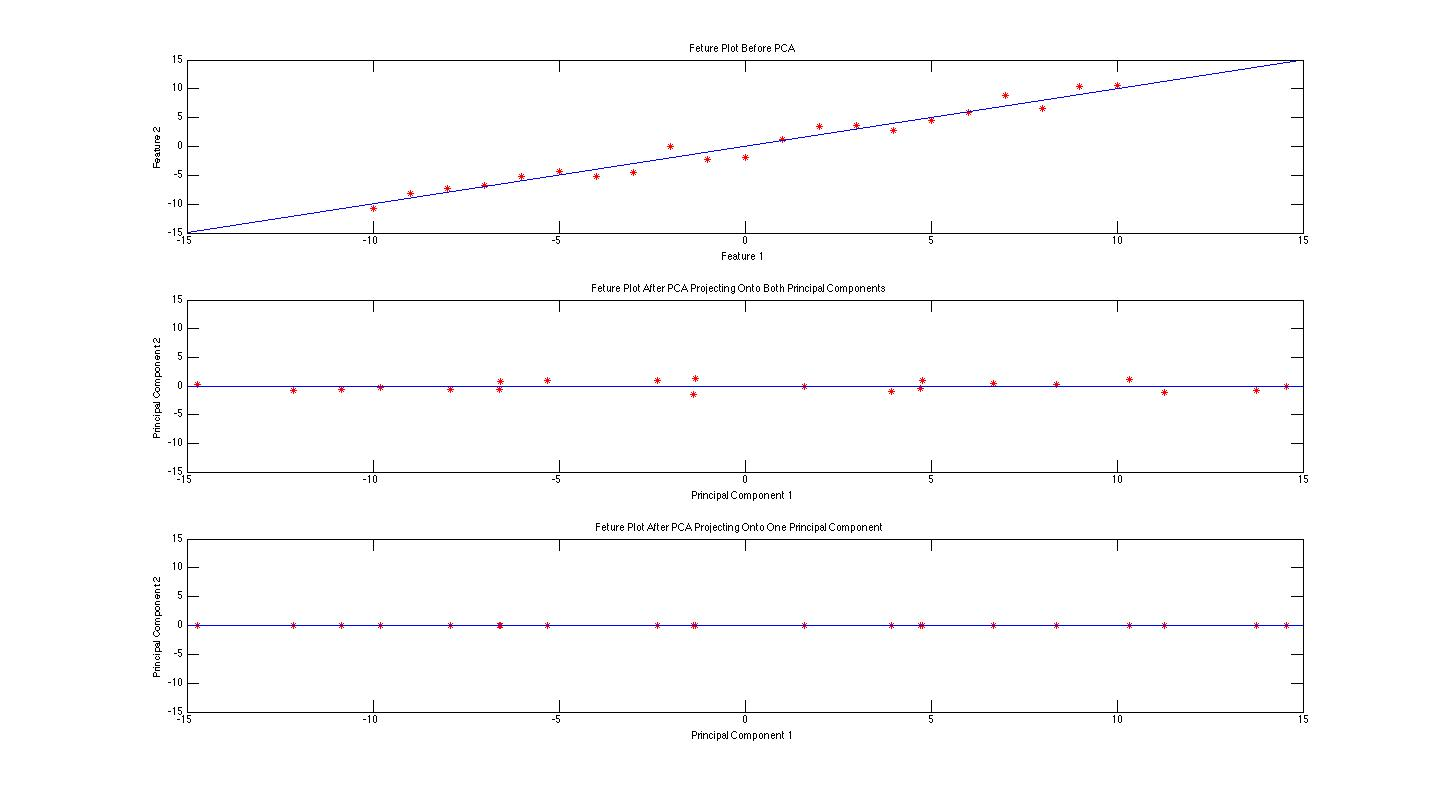
\includegraphics[scale=0.35]{PCA_EXPLAINED.jpg}
\caption{Graphs demonstrating what PCA does. The first graph shows the plot of the features before performing the PCA. The second shows the features projected onto both the new principal components and the third shows the data points only projected onto the first principal component.}
\label{pca}
\end{figure}

\subsection{Similarity to Singular Value Decomposition (SVD)}
This work is largely an extension of \cite{lecture_svd}.

\subsubsection{Description}
SVD is a decomposition method that is very important in many areas due to the way it factorises a matrix into 3 matrices, each with a very informative structure. The basic concept is as such:
\begin{equation}
\mathbf{S} = \mathbf{U}\mathbf{\Sigma}\mathbf{V}^T
\end{equation}
Where $\mathbf{S} \in \mathbb{R}^{m \times n}$,  $\mathbf{U} \in \mathbb{R}^{m \times r}$ and is a column orthonormal matrix, where $r$ is equal to the rank of the matrix,  $\mathbf{V} \in \mathbb{R}^{n \times r}$ is also a column orthonormal matrix, and  $\mathbf{\Sigma} \in \mathbb{R}^{r \times r}$ is a diagonal matrix where the elements are sorted in descending order.

\subsubsection{Example Related to Project}
In the scenario considered in this paper, the matrix $\mathbf{S}$ is a matrix with the rows representing the tweets and the columns representing the words (features). The matrix is made up of only ones and zeros, with $[\mathbf{S}]_{i,j} = 1$, if tweet $i$ contains word $j$ and zero otherwise. As a toy example, suppose we have the matrix:
\begin{equation}
\mathbf{S} = 
\begin{pmatrix}
1 & 1 & 1 & 0 & 0\\
1 & 1 & 1 & 0 & 0\\
1 & 1 & 1 & 0 & 0\\
0 & 0 & 0 & 1 & 1\\
0 & 0 & 0 & 1 & 1\\
0 & 0 & 0 & 1 & 1\\
0 & 0 & 0 & 1 & 1\\
\end{pmatrix}
\end{equation}
Where the columns represent the ordered bag of words, referenced from left to right \{football, cup, win, cyprus, eu\}, and there are two main topics trending on Twitter. One is about some football victory, and the other is about Cyprus joining the EU. This is a very artificial example as it assumes that the tweets would contain the exact same words, but a more general example will be given later. As it can be seen, this matrix is of rank 2, which is also the number of topics that are presented by the matrix. 

Performing the SVD on the matrix, what is acquired is:

\begin{equation*}
\mathbf{S} = \mathbf{U}\mathbf{\Sigma}\mathbf{V}^T
\end{equation*}

\begin{equation}
\mathbf{S} = \begin{pmatrix}
-0.5774 & 0.0000\\
-0.5774 & 0.0000\\
-0.5774 & 0.0000\\
0.0000 & -0.5000\\
0.0000 & -0.5000\\
0.0000 & -0.5000\\
0.0000 & -0.5000\\
\end{pmatrix}
\begin{pmatrix}
3.0000 & 0.0000\\
0.0000 & 2.8284\\
\end{pmatrix}
\begin{pmatrix}
-0.5774 & -0.5774 & -0.5774 & 0.0000 & 0.0000 \\
0.0000 & 0.0000 & 0.0000 & -0.7071 & -0.7071\\
\end{pmatrix}
\end{equation}

These three matrices all have a very significant meaning. It has already been stated that due to the obvious form of $\mathbf{S}$ it can be seen that there are only 2 topics or concepts. The $\mathbf{U}$ matrix can be viewed as the Tweet to concept correlation matrix i.e. how correlated the Tweets are to the corresponding topics. Similarly, the $\mathbf{V}^T$ matrix can be viewed  the concept to word correlation matrix i.e. how related the concept is to the particular word. For example, $\mathbf{U}_{2,1}$ would be how related the second Tweet is to the first concept and $\mathbf{V}^T_{2,3}$ would be how related the second topic is related to the third word, which in this case is zero, i.e. there is no similarity, because the second concept is about Cyprus joining the EU and the third word is win, which does not appear in any Tweet regarding Cyprus and the EU. The $\mathbf{\Sigma}$ matrix is then just the concept strengths.

It can then be shown that $\mathbf{S}^T\mathbf{S}$ represents the correlation of the words in the tweets to each other, i.e. a covariance matrix (see Appendix). But 
\begin{equation*}
\mathbf{S}^T\mathbf{S} = \mathbf{V}\mathbf{\Sigma}\mathbf{U}^T  \mathbf{U}\mathbf{\Sigma}\mathbf{V}^T
\end{equation*}
\begin{equation}
\mathbf{S}^T\mathbf{S} = \mathbf{V}\mathbf{\Sigma}^2\mathbf{V}^T
\end{equation}
which can be rewritten as:
\begin{equation}
\mathbf{S}^T\mathbf{S} = \mathbf{V}\mathbf{\Lambda}\mathbf{V}^T
\end{equation}
which essentially means that the columns of $\mathbf{V}$ are the eigenvectors of the matrix $\mathbf{S}^T\mathbf{S}$ and the diagonal values of $\mathbf{\Lambda}$ are the corresponding eigenvalues, which are the squares of the singular values found in $\mathbf{\Sigma}$.

As it can be seen, there is a close relationship between SVD and PCA, which uses the eigenvectors of the covariance matrix. Therefore, to find the principal components of a matrix $\mathbf{S}$, the SVD can instead be found and the principal components would be the columns of $\mathbf{V}$ (or of $\mathbf{U}$ if we want to find the principal components of $\mathbf{S}\mathbf{S}^T$) and the variances are given by squaring the singular values.

\subsubsection{Further Example Related to Project}
Suppose the matrix $\mathbf{S}$ instead looked like this:

\begin{equation}
\mathbf{S} = 
\begin{pmatrix}
1 & 1 & 1 & 0 & 0\\
1 & 1 & 1 & 0 & 0\\
1 & 1 & 1 & 0 & 0\\
0 & 0 & 0 & 1 & 1\\
0 & 0 & 0 & 1 & 1\\
0 & 0 & 0 & 1 & 1\\
0 & 0 & 0 & 1 & 1\\
1 & 0 & 0 & 1 & 0\\
1 & 1 & 1 & 0 & 0\\
0 & 0 & 0 & 1 & 1\\
0 & 0 & 0 & 1 & 1\\
0 & 0 & 0 & 1 & 1\\
1 & 0 & 0 & 1 & 1\\
\end{pmatrix}
\end{equation}
with the same words representing the columns as in the previous example. It can be seen here that there are now 4 linearly independent columns and therefore this matrix is of rank 4. 

The SVD then turns out to give:


\begin{equation*}
\mathbf{U}=
\begin{pmatrix}
-0.1216&0.4704&-0.1158&0.0223\\
-0.1216&0.4704&-0.1158&0.0223\\
-0.1216&0.4704&-0.1158&0.0223\\
-0.3241&-0.1199&-0.1320&0.0778\\
-0.3241&-0.1199&-0.1320&0.0778\\
-0.3241&-0.1199&-0.1320&0.0778\\
-0.3241&-0.1199&-0.1320&0.0778\\
-0.2336&0.1097&0.7963&0.5471\\
-0.1216&0.4704&-0.1158&0.0223\\
-0.3241&-0.1199&-0.1320&0.0778\\
-0.3241&-0.1199&-0.1320&0.0778\\
-0.3241&-0.1199&-0.1320&0.0778\\
-0.3888&0.0453&0.4363&-0.8102\\
\end{pmatrix}
\end{equation*}
\begin{equation*}
\mathbf{\Sigma}=
\begin{pmatrix}
4.1377&0.0000&0.0000&0.0000\\
0.0000&3.5113&0.0000&0.0000\\
0.0000&0.0000&1.1637&0.0000\\
0.0000&0.0000&0.0000&0.4426\\
\end{pmatrix}
\end{equation*}
\begin{equation*}
\mathbf{V}=
\begin{pmatrix}
-0.2679&0.5801&0.6613&-0.3930\\
-0.1175&0.5359&-0.3980&0.2014\\
-0.1175&0.5359&-0.3980&0.2014\\
-0.6987&-0.1949&0.2654&0.6352\\
-0.6422&-0.2261&-0.4189&-0.6008\\
\end{pmatrix}
\end{equation*}
As it can be seen here, it is significantly more difficult to actually be able to distinguish which words contribute significantly to each principal component due to the added noise that rows 8 and 13 give rise to. This example highlights how important sparse principal components are since here the data is only $\in \mathbb{R}^{13 \times 5}$ and it is already quite difficult to interpret and in a real life scenario these numbers are typically much larger in magnitude, for example, in the scenario considered in this paper this grows to be in the tens of thousands Tweets and thousands of words.

What is very useful to see, however, is that the singular values do decrease quite rapidly after the second one. These represent the square roots of the eigenvalues of the covariance matrix, so by squaring them the graph in Figure \ref{spectrum} is obtained.

\begin{figure}[H]
\centering
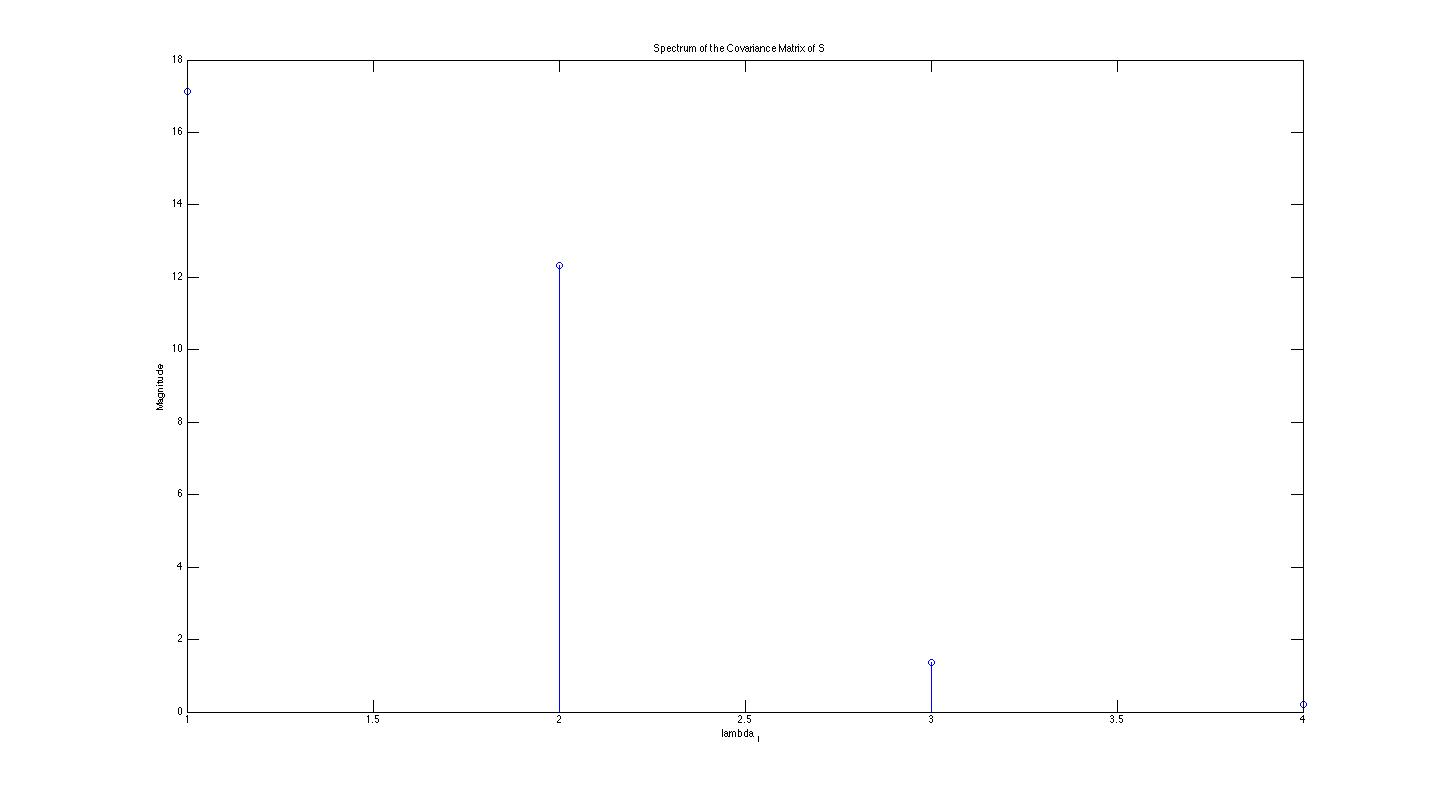
\includegraphics[scale=0.3]{Spectrum_Eigenvalues.jpg}
\caption{The spectrum of the eigenvalues of $\mathbf{S}^T\mathbf{S}$}
\label{spectrum}
\end{figure}

This intuitively makes sense since it is not hard to tell, after looking at the eigenvectors, that the first eigenvector is associated with the words Cyprus and EU, as 7 of the rows only mention these two words from the bag of words. The second eigenvector is associated with the words football, cup and win, as 4 of the rows only contain these words. These are obviously the major concepts and so their eigenvalues are relatively quite high, with the first one being slightly higher. After these however, the eigenvalues fall significantly which relate to the added noise which is present due to the rows 8 and 13, since not much variance can be explained by these two eigenvectors and therefore they carry very little information. 


\subsection{Related Work}
The idea of using social media as a medium for data analysis is not new and much work has been done in this area. Some particular examples are \cite{dimakis} and \cite{microblogs}. These two both lay a solid foundation for the work explored in this paper as it uses a lot of their findings and results and starts where they left off. For instance, the Sparse PCA algorithm that is focused on initially is the same algorithm, with some slight modifications, as in \cite{dimakis} and the data used is the same data as was used in \cite{microblogs}. These both may change as the findings of this project progress, however. The focus of these however is not entirely the same. In \cite{dimakis}, a lot more emphasis is put on the actual algorithm itself, whereas in this paper many other areas are also explored, such as the trade-off between the number of features chosen, the number of points taken and the results obtained. Moreover, scalability is also considered in much more detail than in any of these. 

Furthermore, as mentioned previously, sparse PCA-like algorithms are also an active area of research and as such, much work has been done, some specific examples of which will be explored in this project.

\subsubsection{Sparse PCA}

Sparse PCA algorithms aim to deliver similar results to PCA, but with the difference that they give rise to principal components that only have few non-zero entries. The reason sparsity is desired in the eigenvectors is because sparse approximations of the eigenvectors are useful for interpreting data that have large dimensions. For example, in the specific application discussed in this paper, a set of words is considered and meaningful inferences are to be found from this data. It is clearly much simpler to analyse data given a small set of words that could approximate the variance in the given data set per principal component, than all the words in the data set which would contribute a small amount each, increasing the dimensionality of the principal component to the number of words in the set of all the words in all the Tweets. The equation to be solved resolves to:
\begin{equation}
\mathbf{v}_1 = \underset{\|\mathbf{x}\|_2^2 = 1, \|\mathbf{x}\|_0^2 = k}{\operatorname{argmax}}\left( \mathbf{x}^T\mathbf{A}\mathbf{x}\right)
\end{equation}
where $\|\mathbf{x}\|_0^2$ is the $l_0$ cardinality of $x$ i.e. how many non-zero elements x has. This is where Sparse PCA algorithms come in. 

\subsubsection{Methods to perform Sparse PCA}
Plenty of methods have been designed to get sparse principal components or principal component like vectors, due to the importance of such an algorithm in practice, as detailed above. A few are described here, but by no means do these constitute the full work in this active area of research.
 
The first attempt, and an algorithm that is still widely used regardless of its many limitations is the Thresholding method, which simply performs regular PCA and then forces the entries that are small in magnitude, to zero. This can be misleading and an arbitrary selection of the threshold must be made, which may not actually be valid \cite{cadima}. In \cite{scotlass}, the authors aim to force sparsity by solving the equation
\begin{equation*}
\underset{\substack{\|\mathbf{x}\|_2 = 1, \\ \sum_{j=1}^n|\mathbf{x}| \leq t}}
{\operatorname{argmax}}\mathbf{x}^T\mathbf{A}\mathbf{x}
\end{equation*}
 
for some $t$ where $1<t<\sqrt{n}$, by applying a Lagrange multiplier and then solving a regression type problem. This is done so as to maximise the variance captured by the particular principal component with the constraint that the sum of the entries must be small, which in turn introduces sparsity. This is different to using the $l_2$ norm, which is used in ridge regression and attains variables that are close to, but not exactly, zero and is referred to as the Lasso, which is explained further in \cite{lasso}. Another method which makes use of the Lasso penalty, and various others, can be found in \cite{shen}. This method uses the relationship between Singular Value Decomposition (SVD) and PCA as its basis and but imposes a penalty on the size of the entries in the principal components. Yet another method is known as the Truncated Power Method (TPower), which can be found in \cite{truncpower} and is implemented in this project and used as a benchmark due to its fast performance. This method performs the well known power method for retrieving the dominant eigenvector of a matrix, but keeps the top $k$ values in magnitude and forces the rest to zero upon each iteration till convergence. The problem with many of these methods is that (a) some are quite slow in practice on large data sets, (b) some do not generally guarantee principal components that are orthogonal and so this means that lots of redundancy must also be stored. 

A few more methods must be considered, including \cite{zou}, \cite{daspremont} and \cite{asteris} but have still not been until this point in time. 

\subsection{Sparse PCA through Low-Rank Approximation Algorithm}
This is the algorithm\cite{dimakis} that is most focused on in this paper and for a variety of reasons, which will be mentioned throughout this section, but this may change as the project progresses, if other algorithms prove to be better according to measures that will be defined later. It will be referred to from now on as the Spannogram (Sparse) PCA  algorithm.

\subsubsection{Intuitive Explanation of the Algorithm}
The assumption is made that a rank $d$ approximation of the covariance matrix at hand is arbitrarily close to the original based on the Forbenius norm. That is:

\begin{equation*}
\|\mathbf{A} - \mathbf{A}_d\|_F < \epsilon
\end{equation*}
where $\epsilon$ can be determined. This can then be expressed as:
\begin{equation*}
\mathbf{A}_d = \sum_{i=1}^d \lambda_i \mathbf{v}_i \mathbf{v}_i^T
\end{equation*}

The basic idea behind this algorithm is that the sparse approximation to the first principal component can be found by calculating the eigenvector $\mathbf{x}_*$ with the largest eigenvalue for all the possible $k\times k$ submatrices of $\mathbf{A}$. This leads to finding $n \choose k$ possible sparse eigenvectors, however. This would be quite wasteful however since it would lead to needing to find $O\left( n^k\right)$ eigenvectors, where $k$ is the sparsity of the eigenvector, i.e. how many elements of the vector are non-zero. In \cite{dimakis}, it can be shown that only $O\left(n^d\right)$ candidates need to be examined though and since $d < k$ typically, this means that the time complexity is reduced significantly. This reduction is the result of the Spannogram algorithm described in \cite{dimakis} and the resulting time complexity turns out to be $O \left( n^{d+1}\log(n) + n^d k^2 + dn^2\right)$. Depending on the structure of the matrix $\mathbf{A}$, either one of the terms could prevail.

\subsubsection{The Spannogram Algorithm}

What this algorithm aims to do is eliminate any candidates for the eigenvectors that would be redundant to calculate. The way this can be demonstrated is by taking a Rank-1 matrix, i.e.

\begin{equation*}
\mathbf{A}_1 = \lambda_1 \mathbf{v}_1 \mathbf{v}_1^T
\end{equation*}

and solving the equation

\begin{equation*}
\max_{\substack{\mathbf{x} \in\mathbb{S}_k, \\ \|\mathbf{x}\|_2 = 1, \\ \|\mathbf{x}\|_0 = k}} \mathbf{x}^T\mathbf{A}_1\mathbf{x}
\end{equation*}

where $\mathbb{S}_k$ is the set of all $k$-sparse vectors in $\mathbb{R}^n$. The solution turns out to be:

\begin{equation*}
\lambda_1\max_{\substack{\mathbf{x} \in\mathbb{S}_k, \\ \|\mathbf{x}\|_2 = 1, \\ \|\mathbf{x}\|_0 = k}} \left(\mathbf{v}_1^T \mathbf{x}\right)^2 = \max_{\substack{\mathbf{x} \in\mathbb{S}_k, \\ \|\mathbf{x}\|_2 = 1, \\ \|\mathbf{x}\|_0 = k}} \lambda_1\left( \sum_{i = 1}^n [\mathbf{v}_{1}]_i [\mathbf{x}]_i\right)^2
\end{equation*}

Therefore, it can easily be seen that just by keeping the $k$ entries with the largest magnitude and making all other entries equal to 0 in x would satisfy the equation above. Therefore, the solution is trivial. 

For the case where $d > 1$, what the algorithm essentially does is transform the problem into many Rank-1 case problems and solve them to find the best solution.

The eigenvectors of $\mathbf{A}_d$, which can be represented as:
\begin{equation*}
\mathbf{V}_d = [\sqrt{\lambda_1}\mathbf{v}_1, \cdots, \sqrt{\lambda_d}\mathbf{v}_d]
\end{equation*}

\begin{equation*}
\max_{\substack{\mathbf{x} \in\mathbb{S}_k, \\ \|\mathbf{x}\|_2 = 1, \\ \|\mathbf{x}\|_0 = k}}  \mathbf{x}^T\mathbf{A}_d\mathbf{x} = \max_{\substack{\mathbf{x} \in\mathbb{S}_k, \\ \|\mathbf{x}\|_2 = 1, \\ \|\mathbf{x}\|_0 = k}} \|\mathbf{V}_d^T\mathbf{x}\|_2^2
\end{equation*}


It then defines a vector, $\mathbf{c} \in \mathbb{R}^d$ such that $\|\mathbf{c}\|_2=1$, which is a function of some vector $\mathbf{\phi}$ and the elements in it are sinusoids taking as arguments the elements in $\mathbf{\phi}$, where each $\phi_i \in (\frac{-\pi}{2}, \frac{\pi}{2}]$.

The equation is then transformed into a Rank-1 instance by creating the vector $\mathbf{u}_c = \mathbf{u}_d \mathbf{c}$ to give 

\begin{equation}
\max_{\|\mathbf{c}\|_2 =1} \max_{\substack{\mathbf{x} \in\mathbb{S}_k, \\ \|\mathbf{x}\|_2 = 1, \\ \|\mathbf{x}\|_0 = k}}\left(\mathbf{v}_c^T \mathbf{x}\right)^2 
\label{spannogram}
\end{equation}

Therefore, when $\mathbf{c}$ is fixed there is a simple trivial solution to  equation \ref{spannogram}. The important thing to note is that, there is no actual need to calculate the actual value of the $\mathbf{v}_c$ for each $\phi$ to find the candidate indices for the $k$-sparse eigenvectors only the relative magnitudes between the different entries in  $\mathbf{v}_c$ must be taken into account. The relative magnitudes will only change at intersection points between the sinusoids, and therefore, only about these points must a candidate eigenvector indices actually be tested. This brings down the computation to $O \left(n^d\right)$ instead of $O \left(n^k\right)$. A more thorough description and justification of the algorithm can be found in \cite{dimakis}.

\subsubsection{Other Benefits}
Other reasons this algorithm has been chosen is because the authors of \cite{dimakis} claim it has a safe feature elimination procedure which results in a significant improvement to the computation time and is based on the Spannogram Algorithm described above. Also, if $\mathbf{A}$ consists of only positive entries, which it does in our case, the algorithm speeds up by a factor of $2^d$, which further brings down the time complexity. Another great feature it has is that the principal components found are also orthogonal to each other meaning that less redundancy has to be stored, which is based on the projection deflation method described in \cite{Mackey_deflationmethods}. 
\clearpage
\section{Completed Implementation}

\subsection{The Bag-of-Words}
The choice of words to be chosen as the features must be carefully considered. For instance, one could simply take a union of all the words in the English dictionary, the words that are used on the internet, such as ``lol'' and ``yey'', and all the possible names of people and places, which would solve the problem of possibly missing out any features. This however would result in a matrix of immense dimension and therefore would be impossible to process, at least given any consumer computer. Therefore, some careful selection for the features must be exhibited so as to gain the features that carry the most information whilst still keeping the number of features to a manageable size. Some general guidelines for all methods are that words that typically do not give any additional information e.g. ``is'', ``the'', ``this'', etc. are to be eliminated. Furthermore, the Bag-of-Words should be completely independent of case i.e. ``Road'' and ``road'' are to be considered equal. 

\subsubsection{Using Set of All Words in Tweets}
This first method attempts to use all the words that appear in the Tweets with the filter described above applied. Unfortunately, this results a set of over 78,000 features, which is much to large to process, so this method is not to be used. 

\subsubsection{Using Set of Three Thousand Most Common Words in the English Language}
The next method is to use a set of the 3,000 most common words in the English language as a whole. A problem with this is that, this list typically includes a lot of the very uninformative words, examples of which are given above, and does not include words that are not very common as a whole but, when some sort of event occurs, become very common, especially on social media. Furthermore, it also does not include any names or slang that is used on the internet. To illustrate, if Muse were to have a concert some time in June, it would be expected that a lot of Tweets may have the word ``Muse'' in them and ``concert'' and words like ``wow'' or ``amazing'', all of which are not in the top 3,000 words in the english language. Therefore, these features would be completly missed out and therefore a very valid principal component would possibly be non-existent in the final results.

\subsubsection{Adding Words in Tweets to the Bag-of-Words with a Certain Probability}
Another approach is to say that a word is added to the Bag-of-Words with a probability $p$. The intuition behind this is that words that do appear very often most probably will end up in the set, if p is large enough, but of the words that do not appear very often there would be less, giving a much more relevant bag of words and a much smaller set also (approximately $p$ times the size of the original).

We assume that all words are independent. Let $T_w$ be the event that we take the word $w$ and $A_{w, i}$ be the event that the word $w$ appears $i$ times and assume the probability of taking a word $w$, given that $w$ appears is $p$. 
\begin{equation*}
P\left( T_w | A_{w, i}\right) =  \sum_{j=1}^i {i \choose j} p^j\left( 1 - p\right)^{i-j}
\end{equation*}
which is equivalent to 
\begin{equation}
P\left( T_w | A_{w, i}\right)  = 1 - P(\bar{T}_w |  A_{w, i}) = 1 - (1 - p)^i
\end{equation}

We can therefore see that the higher the occurrence of the word $w$, the higher the probability of it being added to the Bag-of-Words. Since popular events will have words associated with them that appear quite often, it can be said that with the right choice of $p$, more informative words will appear in the Bag-of-Words, whilst also reducing the size of the set. 

This gives a final algorithm that is $O(N)$, where $N$ resembles the number of all the unique words in all the Tweets. 

This method seems to work to some extent, however, if the set of all the words grows too large, the probability $p$ will have to become much smaller to maintain a constant size for the Bag-of-Words. In turn, this means that the relevant words would have to occur more for them to be in the final set. This may not be the case however if taken over longer periods of time in which words associated with events may have large spikes for a few hours or days but when taken over the whole period of time, actually contribute a small percentage of the whole set of words.

\subsubsection{Taking $M$ Words of Highest Occurrence}

In this case, a set of words is created as before, but the frequency of each word in the set is also counted and the words are sorted in descending order of occurrence. When this is done, the first $M$ words are taken as the Bag-of-Words. The assumption here is that words that appear very often will be in the principal components, which is not completely justified, but empirically has been the case. For example, having taken the top 3000 words, the principal components always have words in the top 1000 words, most of which are in the top 500. This makes the computation feasible whilst still not losing a significant amount of information.

This is a $O(NlogN)$ algorithm, where $N$ resembles the number of all the unique words in all the Tweets. 

This suffers from the same problem as the probabilistic method, however, it ensures that words that do occur very frequently will be in the Bag-of-Words, as opposed to relying on probability. This method will be used from now on in this paper.

\subsection{The Matrix $\mathbf{A}$}
\label{covmat}

The matrix to be passed to the Sparse PCA algorithm is also of interest, as it determines what sort of relationship the words have to one another. In this section, different versions of the matrix are considered and evaluated against each other so as to be used from here on. 

All testing is done using a subset of the Tweets, namely the first 1000 Tweets. This is roughly a day's worth of data. The Spannogram Algorithm\footnote{Note that the Spannogram Algorithm itself has not yet been evaluated but is taken to work well enough as an assumption which is based on \cite{dimakis}} is run on each of the matrices using the same parameters and 3 5-sparse PCAs are computed.
\subsubsection{The Initial Matrix $\mathbf{A}$}
The matrix which the sparse principal components are extracted from may take many forms. Initially, the approach considered in \cite{dimakis} is taken, in which $\mathbf{A} = \mathbf{S}^T \mathbf{S}$ where $\mathbf{S} \in \mathbb{R}^{m \times n}$ is the data matrix with $m$ rows as the Tweets and $n$ columns representing each of the words in the Bag-of-Words. However, different methods may also be explored which change the weightings of the features. 

\subsubsection*{Results}
\begin{table}[H]
\center
\begin{tabular}{| c l | c l | c l |}
\hline
Index & Word & Index & Word & Index & Word\\
\hline
2 & love & 3 & london & 1 & like\\
6 & know & 83 & hall & 9 & back\\
4 & people & 77 & royal & 44 & feel\\
1 & like & 9 & back & 13 & going\\
7 & don't & 166 & albert & 15 & follow\\
\hline
Eigenvalue & 44.4 & Eigenvalue & 35.1 & Eigenvalue & 33.1\\
\hline
\end{tabular}
\caption{The first 3 principal components using the algorithm on the initial matrix, $ \mathbf{A}$. The index represents the rank of the word according to how frequent the word is found in the all the tweets. The associated eigenvalue is also shown for each of the principal components.}
\end{table}

As it can be seen, two of the three principal components in this case do not really convey much information as to any particular event that took place and are just words that may be used together quite often but not especially when a certain event takes place, however the middle one does seem to give some insight. It seems to indicate that during the time these Tweets were created there was an event at the Royal Albert Hall in London. 

The eigenvalues also give some good insight and are useful for scoring the importance of different principal components. The higher the eigenvalue, the higher the variance this principal component accounts for, and therefore the more information it holds. In this scenario, the second principal component seems to get the second highest eigenvalue, which should be noted for the next case. 
  
\subsubsection{The Hollow Matrix $\mathbf{A}_{h}$}
As described in Appendix A, the matrix $\mathbf{A} = \mathbf{S}^T \mathbf{S}$ can be viewed as an undirected graph with each node being a word and each link being the number of times that word appears with the connecting word node in the same Tweet for all Tweets. This representation is meaningful, however the problem lies in the fact that the diagonal represents the number of times each word appears in total, regardless of any relation to the other words i.e. each node has a link to itself, with the highest weighting. This means that words that occur very frequently have very large values on their diagonal, regardless of how they relate to other words, which can be deceiving when taking the eigenvalues of the matrix. In attempt to prevent this, the matrix $\mathbf{A}$ can be substituted for 
$\mathbf{A}_h$ where for each of its elements, $[\mathbf{A}']_{i, j}$, it takes the value 

\begin{equation}
[\mathbf{A}']_{i, j}= 
\begin{cases}
[\mathbf{A}]_{i, j} & \text{if}\ i \neq j\\
0 & \text{if}\ i = j
\end{cases}
\end{equation}

\subsubsection*{Results}
\begin{table}[H]
\center
\begin{tabular}{| c l | c l | c l |}
\hline
Index & Word & Index & Word & Index & Word\\
\hline
6 & know & 13 & going & 3 & london\\
7 & don't & 22 & some & 83 & hall\\
1 & like & 14 & sleep & 77 & royal\\
16 & about & 52 & **** & 166 & albert\\
4 & people & 102 & house & 124 & greater\\
\hline
Eigenvalue & 13.5 & Eigenvalue & 9.6 & Eigenvalue & 16.6\\
\hline
\end{tabular}
\caption{The first 3 principal components using the algorithm on the hollow matrix, $ \mathbf{A}_h$. The index represents the rank of the word according to how frequent the word is found in the all the tweets. The associated eigenvalue is also shown for each of the principal components.}
\end{table}

In this case, once again two of the three principal components are not very insightful but the third is again talking about the Royal Albert Hall in London. The interesting thing to not here is that the associated eigenvalue for the third principal component and the most useful is actually the highest. This, as suspected, means that this method gives significantly better results that the previous method.

\subsubsection{The Normalised Matrix $\mathbf{A}_{n}$}
Here, making the matrix have normalised rows is considered and the resulting matrix is $\mathbf{A}_n$. The basic concept is to make it so that all the rows/columns sum to 1 so that it does not matter which words actually appear the most, but how often they appear with other words relative to their weighting.

\subsubsection*{Results}

\begin{table}[H]
\center
\begin{tabular}{| c l | c l | c l |}
\hline
Index & Word & Index & Word & Index & Word\\
\hline
1782 & glisse & 2084 & cried & 1615 & iwalnut\\
1484 & mafia & 1692 & hollyoakslater & 2339 & arre\\
773 & volton & 873 & tonight's &2422 & abrazo\\
1008 & sons & 2382 & alkolik & 1351 & olmaden\\
2086 & conette & 900 & throuhout & 1711 & hermano\\
\hline
\end{tabular}
\caption{The first 3 principal components using the algorithm on the hollow matrix, $ \mathbf{A}_n$. The index represents the rank of the word according to how frequent the word is found in the all the tweets. }
\end{table}

Clearly this gives results that are absolutely irrelevant. The reason for this is because, now that all the words have been normalised, those that appear only a few times together with other words will get a higher weighting. For instance, if a word $a$ only appears once with another word $b$ and never with any other word in the bag of words, then it will get a value of 1 and, therefore will appear to give a higher variance than it does in actual fact. This method will not be considered from here on.

\subsection{Scalability}
Until this point, the matrix $\mathbf{S} \in \mathbb{R}^{m \times n}$, where $m$ is the number of tweets and $n$ is the number of words in the bag of words, has to be very limited in size. This may work for the area of London as 40k Tweets corresponds to roughly a whole day, but if a larger area is considered, this may not correspond to enough time to give any meaningful results. For instance,  there are on average 58 million tweets per day worldwide,\cite{statbrain} 40k of this corresponds to only $0.069\%$ of all the Tweets, which in turn corresponds to about 1 minute of Tweets. It is obvious that this will not give relevant results and so a solution must be found to scale this algorithm and give approximate values for $\mathbf{S}$ such that the processing will be feasible with some arbitrary error. 

\subsubsection{Taking Advantage of the Sparsity of the $\mathbf{S}$ Matrix}
\label{sparsity_matrix}

Taking the current dataset as an example, there are over 40k data points (the Tweets) and, in the best case scenario, roughly 2000 features (the set of words to be evaluated against). This gives a matrix $\mathbf{S}$ of dimension $40k\times 2000$. 
The maximum number of elements that could possibly be non-zero in each row is 28 (since there is a 140 character limit per Tweet and if a average word length of 5 is used, this gives roughly 28 words per Tweet) giving a total of 28 non-zero elements of 2000 per each row, a mere $1.4\%$ of the total entries and this is wildly overestimated since it is probable that most of the Tweets will not reach the 140 character limit and for those that do, only some of their words will be in the chosen bag of words. It can therefore be seen that the matrix will be very sparse, consisting of less than $1.4\%$ non-zero entries.

This is very useful to know beforehand, as one of the limiting factors in this whole method is the memory requirement, but taking advantage of the sparsity of the matrix, we know that at least $98.6\%$ of the matrix will not need to be stored as it will be all zeros. Fortunately, Matlab has an implementation of sparse matrices, which can be used to save a vast amount of space and all the operators that work on regular matrices also apply to sparse matrices as well. Using these, it has been possible to realise the method, with the same results as before, for a matrix $\mathbf{S} \in \mathbb{R}^{286k\times5k}$, which is much larger than the previous limit of about $\mathbf{S} \in \mathbb{R}^{50k\times3k}$.

\subsubsection{Reducing the Dimensionality of $\mathbf{S}$}
The data matrix $\mathbf{S} \in \mathbb{R}^{m \times n}$, where $m$ is the number of tweets and $n$ is the number of words in the bag of words, should be transformed to a lower dimensional space to give $\mathbf{S}_{new} \in \mathbb{R}^{k \times n}$ is the new data matrix where $k << m$. $\mathbf{S}_{new}$ should be a reduced dimension approximation of  $\mathbf{S}$, such that:


\begin{equation*}
0 \le ||\mathbf{S}_{new}^T\mathbf{S}_{new} - \mathbf{S}^T\mathbf{S}|| \le \epsilon 
\end{equation*}

for some arbitrary $\epsilon$. Note that a variant of $\mathbf{A} = \mathbf{S}_{new}^T\mathbf{S}_{new}$ is what will be passed into the Sparse PCA algorithm. 

Methods of this form will be considered further, if needed, but will not be the focus at this point in time.

%\subsubsection*{Frequent-Directions Method}
%This method is described in detail in \cite{edo}. 
%\textbf{Discuss further with supervisor and ask questions in exercise book before writing about this.}
%\subsubsection*{Random Projection Method}
%In this method, one tries to find a matrix  $\mathbf{P} \in \mathbb{R}^{k \times m}$, such that:

%\begin{equation*}
%\mathbf{S}_{new} = \mathbf{P}\mathbf{S} 
%\end{equation*}

%where $\mathbf{S}_{new} \in \mathbb{R}^{k \times n}$ is the new data matrix where $k << m$. \textbf{Provide reference to paper where random projection is used with Gaussian matrix.}

%The problem with the direct implementation in practice is that, in order to get $\mathbf{S}_{new}$, $\mathbf{S}$ must first be loaded into memory, which is exactly what needs to be avoided in the first place. The way to work around this is to tweak this equation so that it can be done on disk, without having to move everything into memory. This gives rise to:

%\begin{equation*}
%\mathbf{S}_{new}^T = \mathbf{S}^T\mathbf{P}^T 
%\end{equation*}

%\begin{equation*}
%\mathbf{s}_{new, i}^T = \mathbf{s}_{i}^T\mathbf{P}^T 
%\end{equation*}

%where $\mathbf{s}_{new, i}^T \in \mathbb{R}^{1 \times k}$ and $\mathbf{s}_{i}^T \in \mathbb{R}^{1 \times m}$ are the $i$th rows of $\mathbf{S}_{new}^T$ and $\mathbf{S}^T$ respectively. This now results to just reading in line by line the file containing $S^T$ from disk storage, which is completely feasible. The resulting matrix $\mathbf{S}_{new}^T$ has $n$ rows corresponding to the bag of words projected onto a lower dimension $k$ of Tweets.

%More on random projections can be found in \cite{randomprojections}.
 
\clearpage

\section{Evaluation of Algorithms}
\subsection{Measuring Performance of Sparse PCA Algorithms}

\subsubsection{Cumulative Percentage of Explained Variance (CPEV)}
Various metrics could be defined as to what good approximations to the principal components using sparse PCA would need to fulfill, but what is generally agreed upon is that the variance captured by each sparse principal component should be maximised and this can be measured by the absolute value of the eigenvalue associated with that eigenvector. When calculating the cumulative variance captured by multiple sparse principal component, however, the difficulty arises that many sparse PCA algorithms do not generally return orthogonal principal components. This in turn means that just by summing the eigenvalues associated with them to get the integrated variance captured by the $k$ principal components does not generally give the right result, as many of the principal components share information leading to an overestimate of the cumulative variance captured. Namely, the following formula, found in \cite{dimakis}, to find the proportion of variance captured by the $k$ principal components will not work for most of the algorithms tested in this section:

\begin{equation*}
v = \frac{\sum_{i=1}^3\lambda^{(c)}_i}{\sum_{i=1}^3\lambda^{(a)}_i}
\end{equation*}
where the superscript $c$ denotes the calculated value, using one of the sparse PCA algorithms, and $a$ is for the actual value.

The measure used in this paper is the same as in \cite{shen}. The centred data matrix is first projected onto the subspace spanned by the $k$ principal components, using the following formula:

\begin{equation}
\mathbf{S}_k = \mathbf{S}\mathbf{\hat{V}}\left(\mathbf{\hat{V}}^T\mathbf{\hat{V}}\right)^{-1} \mathbf{\hat{V}}^T
\label{captured_var}
\end{equation}

where $\mathbf{\hat{V}}$ represents the matrix whose columns are the principal components calculated using any given algorithm. The variance captures is then given by $\Tr\left( \mathbf{S}_k^T\mathbf{S}_k\right)$. It can be seen that when the principal components calculated are orthogonal then $\mathbf{\hat{V}}$ is also orthogonal and therefore $\mathbf{\hat{V}}^T\mathbf{\hat{V}} = \mathbf{I}$ and what is attained is:

\begin{equation}
\mathbf{S}_k =\mathbf{\hat{U}} \mathbf{\hat{\Sigma}}\mathbf{\hat{V}}^T
\label{captured_var}
\end{equation}
 
which is the calculated singular value decomposition of the projected data matrix and the cumulative explained variance can be given by:

\begin{equation*}
\sum_{i=1}^k [\mathbf{\Sigma}]_{i,i}^2 
\end{equation*}

In general, to find the proportion of variance captured by the $k$ principal component, the equation used is:

\begin{equation}
v_\text{cepv} = \frac{\Tr\left( \mathbf{S}_k^T\mathbf{S}_k\right)}{\Tr\left( \mathbf{S}^T\mathbf{S}\right)}
\end{equation}

and has a value between 0 and 1. This quantity is referred to as the cumulative percentage of explained variance (CPEV) in \cite{shen} and shall be referred to as such here also. 


\subsubsection{Sparsity}
Another obvious measure of performance, is the sparsity level which is attained by the algorithm. If a desired sparsity is stated, then the algorithm should be able to attain close to that and if it doesn't, the performance should decrease. 

\subsubsection{Objective Function for Performance}
The objective function for the performance for each algorithm is therefore given as a result of these measurements. It is chosen arbitrarily but with good reasoning. The formula is given by:

\begin{equation}
P = v_\text{cepv} - \gamma \left(k - \hat{k}\right)^2
\label{obj_function}
\end{equation}
where, $P$ is the performance score, $k$ is the desired sparsity and $\hat{k}$ is the actual sparsity returned. $\gamma$ is a tuning parameter and is the penalty multiplier for the difference in the desired sparsity versus the actual sparsity. 







\subsection{Testing the Sparse PCA Algorithms on Artificial Data}\label{testing}
\subsubsection{Testing with Sparse Principal Components}
The first way the algorithms are tested in this project, is by creating an artificial $n \times n$ covariance matrix with 3 known sparse principal components with their respective eigenvalues, as described in \cite{truncpower} and \cite{shen}. 

The 3 eigenvectors alongside their eigenvalues, are chosen to be:

\begin{equation*}
[\mathbf{v}_1]_i = \begin{cases}
       \frac{1}{\sqrt{5}} & \text{, for } 1<i\le 5 \\
       0 & \text{, else }
        \end{cases}
        \text{              , } \lambda_1 = 5
\end{equation*}
\begin{equation*}
[\mathbf{v}_2]_i = \begin{cases}
       \frac{1}{\sqrt{5}} & \text{, for } 5<i\le 10  \\
       0 & \text{, else }
        \end{cases}
        \text{              , } \lambda_2 = 3
\end{equation*}
\begin{equation*}
[\mathbf{v}_3]_i = \begin{cases}
       \frac{1}{\sqrt{5}} & \text{, for } 10<i\le 15  \\
       0 & \text{, else }
	  \end{cases}  
	  \text{              , } \lambda_3 = 2  
\end{equation*}
       
these are then put into columns along with two other eigenvectors orthogonal to each other and in the null space of $[\mathbf{v}_1 \mathbf{v}_2 \mathbf{v}_3]$ with random entries, which have associated eigenvalues of smaller magnitude than these three, to create an orthonormal set. This gives $\mathbf{V}$ and the eigenvalues are stacked into a diagonal matrix to give $\mathbf{\Lambda}$. The covariance matrix, is then created, as such:

\begin{equation*}
\mathbf{A} = \mathbf{V}\mathbf{\Lambda}\mathbf{V}^T
\end{equation*}


Then $m$ data points are drawn from a  zero mean multivariate Gaussian distribution  with this covariance matrix as a parameter to give $\mathbf{S} \in \mathbb{R}^{m \times n}$. The sample covariance matrix is then calculated by:

\begin{equation*}
\mathbf{\hat{A}} = \frac{1}{m}\left(\mathbf{S} - \bar{\mathbf{S}}\right)\left(\mathbf{S} - \bar{\mathbf{S}}\right)^T
\end{equation*}
where $\bar{\mathbf{S}}$ is a vector of the sample means of every feature.

Then the Sparse PCA algorithms are used on this covariance matrix to find the approximated principal components. This is repeated 10 times varying the signal to noise ratio (SNR), which is calculated as:

\begin{equation*}
\text{SNR} = \frac{\sum_{i = 1}^3\lambda_i^{(a)}}{\sum_{i = 4}^5\lambda_i^{(a)}2^{(j-1)}}
\end{equation*}

where $\lambda_i^{(a)}$ denotes the actual eigenvalue of the $i$th eigenvector, the first three being the sparse ones and the last two being the noise components, and $j$ denotes the iteration number (starting from 1). As it can be seen the SNR will decrease with each iteration number, as the eigenvalues of the noise eigenvectors increase by a factor of two upon each iteration. This is done for $m=5000$ data points and then for $m=10$ data points and is iterated 10 times for each, averaging the outcome. 

The algorithms used are the Spannogram algorithm in \cite{dimakis} with a rank 3 approximation, which is referred to as Spannogram-R3; the TPower method in \cite{truncpower} and the Generalised Power Method method described in \cite{GPower} with the $l_1$ and the $l_0$ penalties, referred to as GPower-$l_1$ and GPower-$l_0$ respectively.

\begin{table}[H]
\center
\begin{tabular}{|l|r|r|r|}
\hline
Algorithm &  CPEV Max & CPEV Min & Average Computation Time/s\\
\hline
Spannogram-R3 & 0.8636  & 0.1420&9.8973\\
TPower &  0.9992 &  0.7100&0.0106\\
GPower-$l_1$ &0.9992 & 0.6417& 0.0301\\
GPower-$l_0$ &0.9992 & 0.6370& 0.0148\\
\hline

\end{tabular}
\caption{Table showing the performance of different algorithms for computing sparse principal components of the covariance matrix $\mathbf{A}$ with $m=5000$.}
\label{performance_5000}
\end{table}

\begin{table}[H]
\center
\begin{tabular}{|l|r|r|r|}
\hline
Algorithm &  CPEV Max & CPEV Min & Average Computation Time/s\\
\hline
Spannogram-R3 &  0.9067 & 0.4699&9.8415 \\
TPower &  0.9992 &  0.7180&0.0137\\
GPower-$l_1$ &0.9992 & 0.8641& 0.0034 \\
GPower-$l_0$ &0.9992 & 0.7468 &0.0013\\
\hline

\end{tabular}
\caption{Table showing the performance of different algorithms for computing sparse principal components of the covariance matrix $\mathbf{A}$ with $m=10$.}
\label{performance_10}
\end{table}

\begin{figure}[H]
\centering
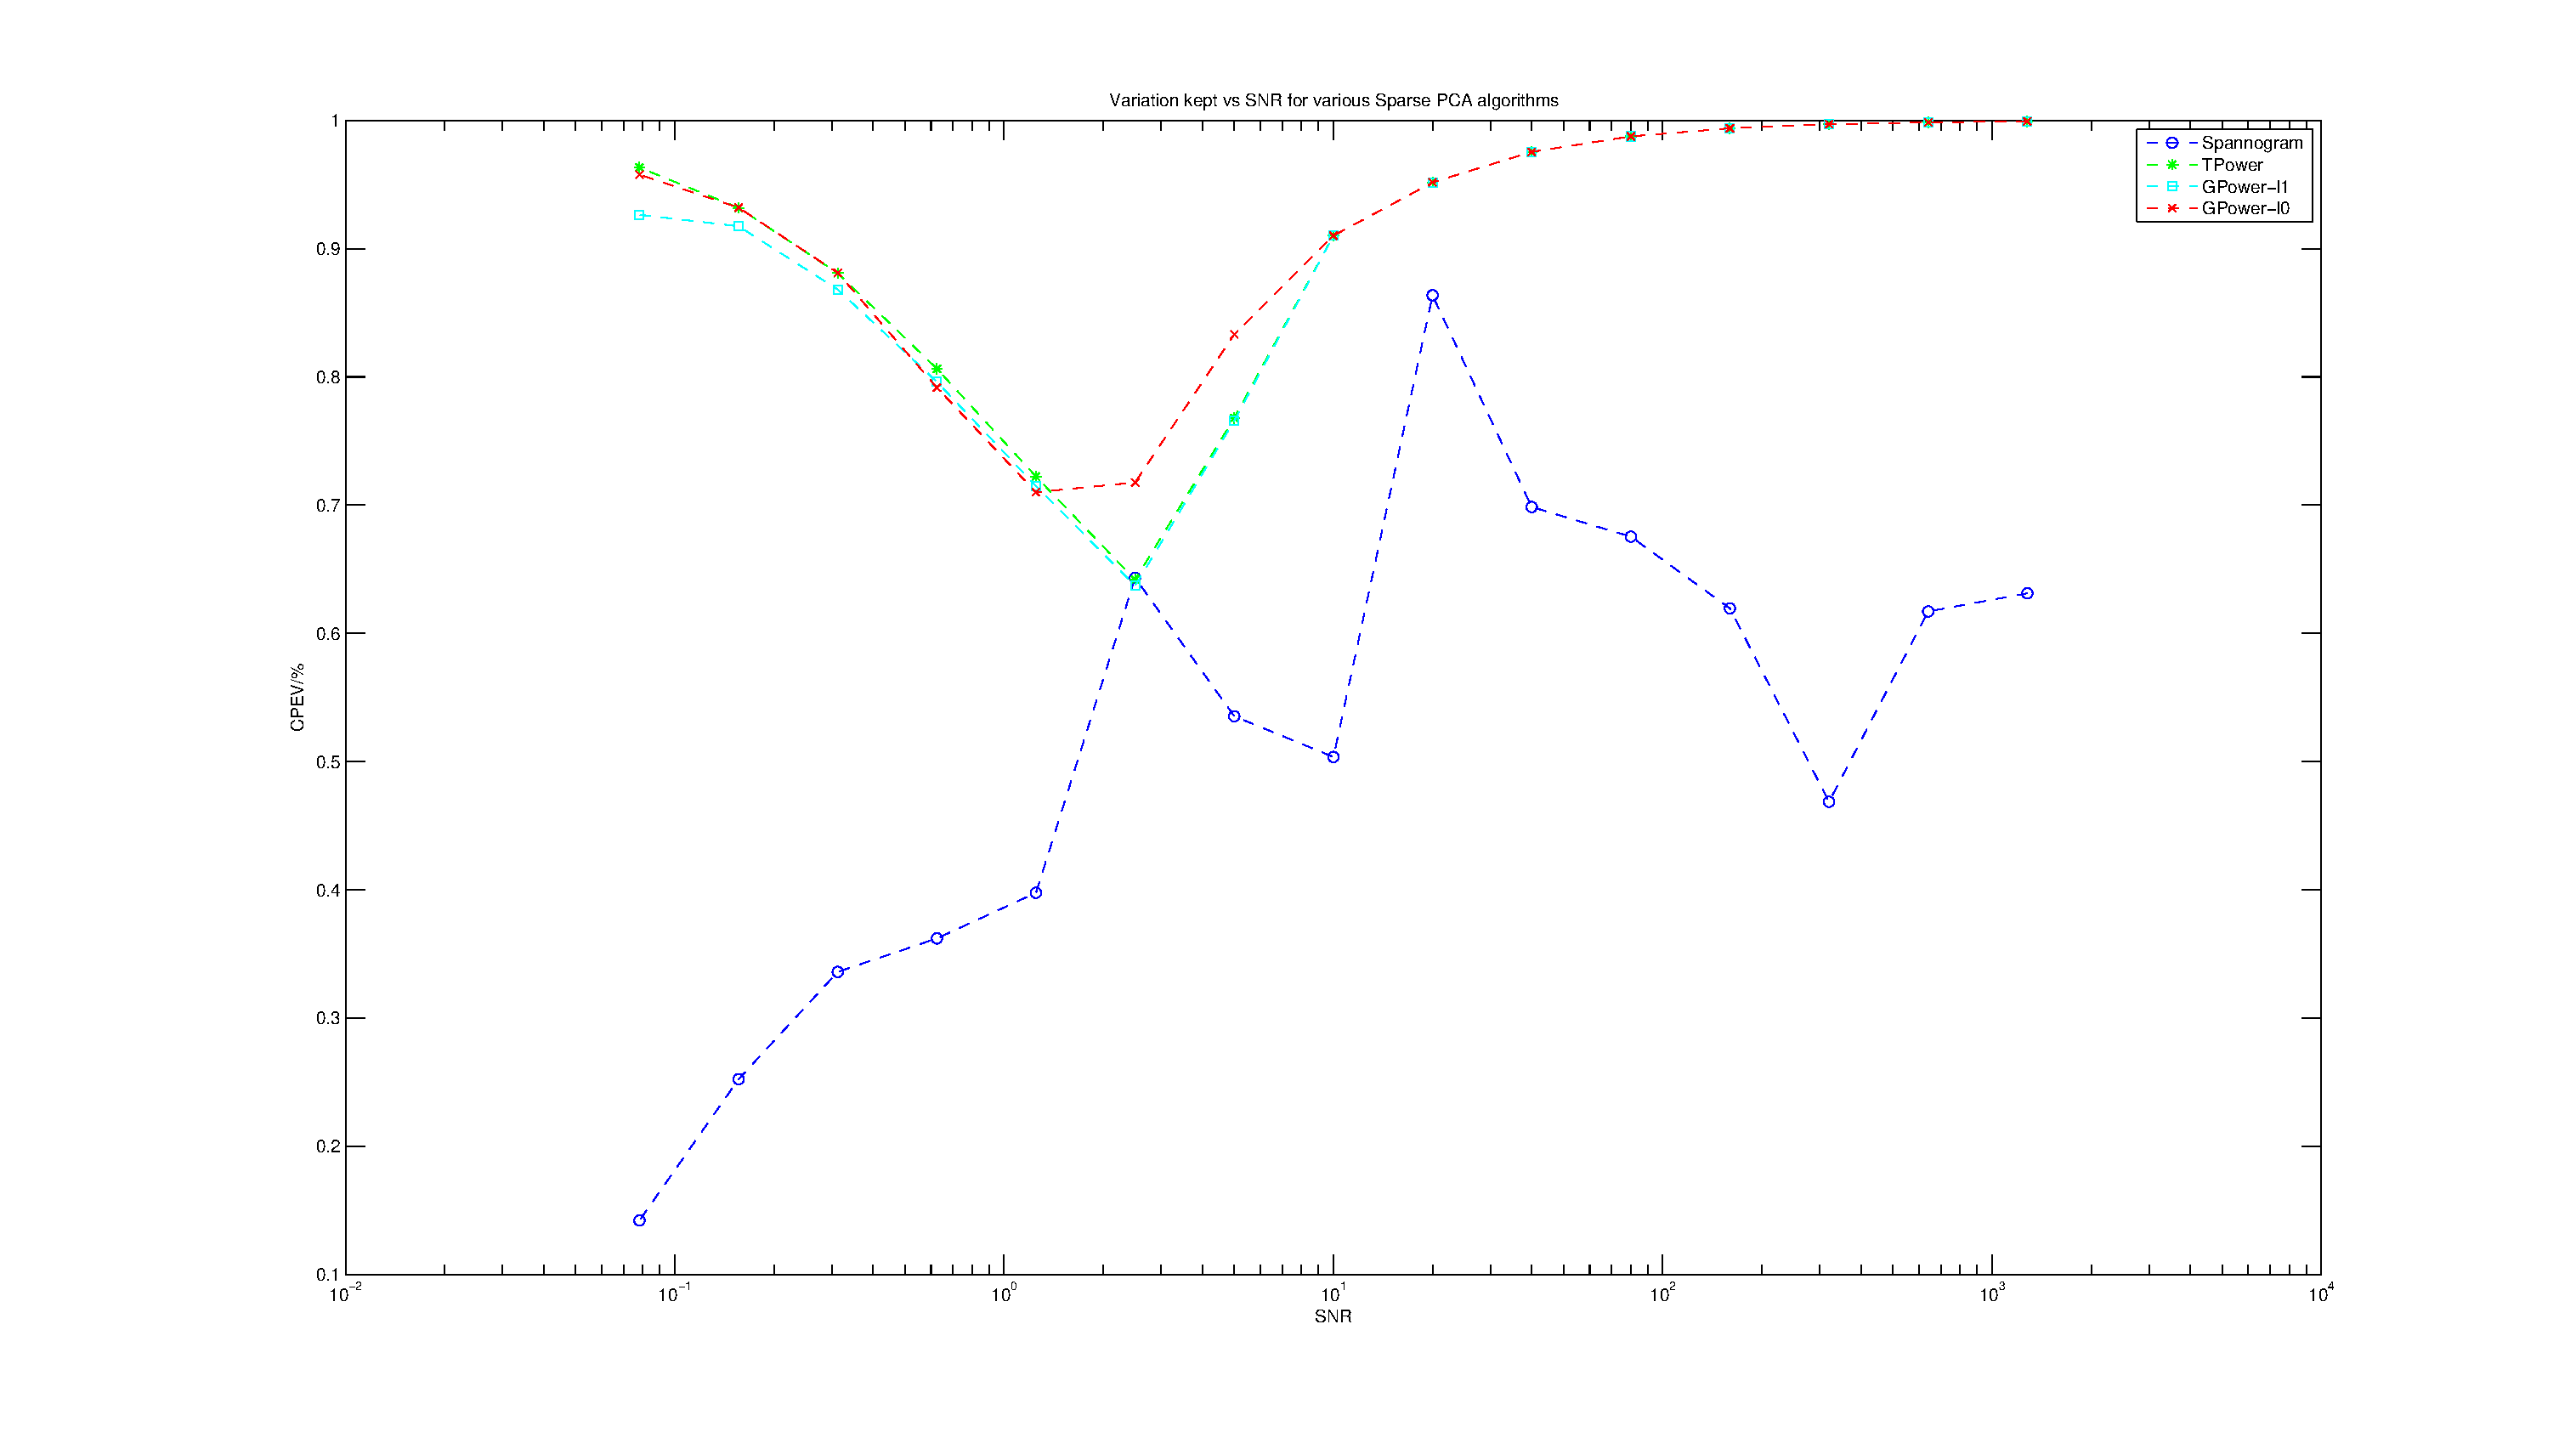
\includegraphics[scale=0.3]{CPEV.eps}
\caption{How the different algorithms perform as the SNR varies for fixed sparsity with $m = 5000$.}
\label{cpev_5000}
\end{figure}

\begin{figure}[H]
\centering
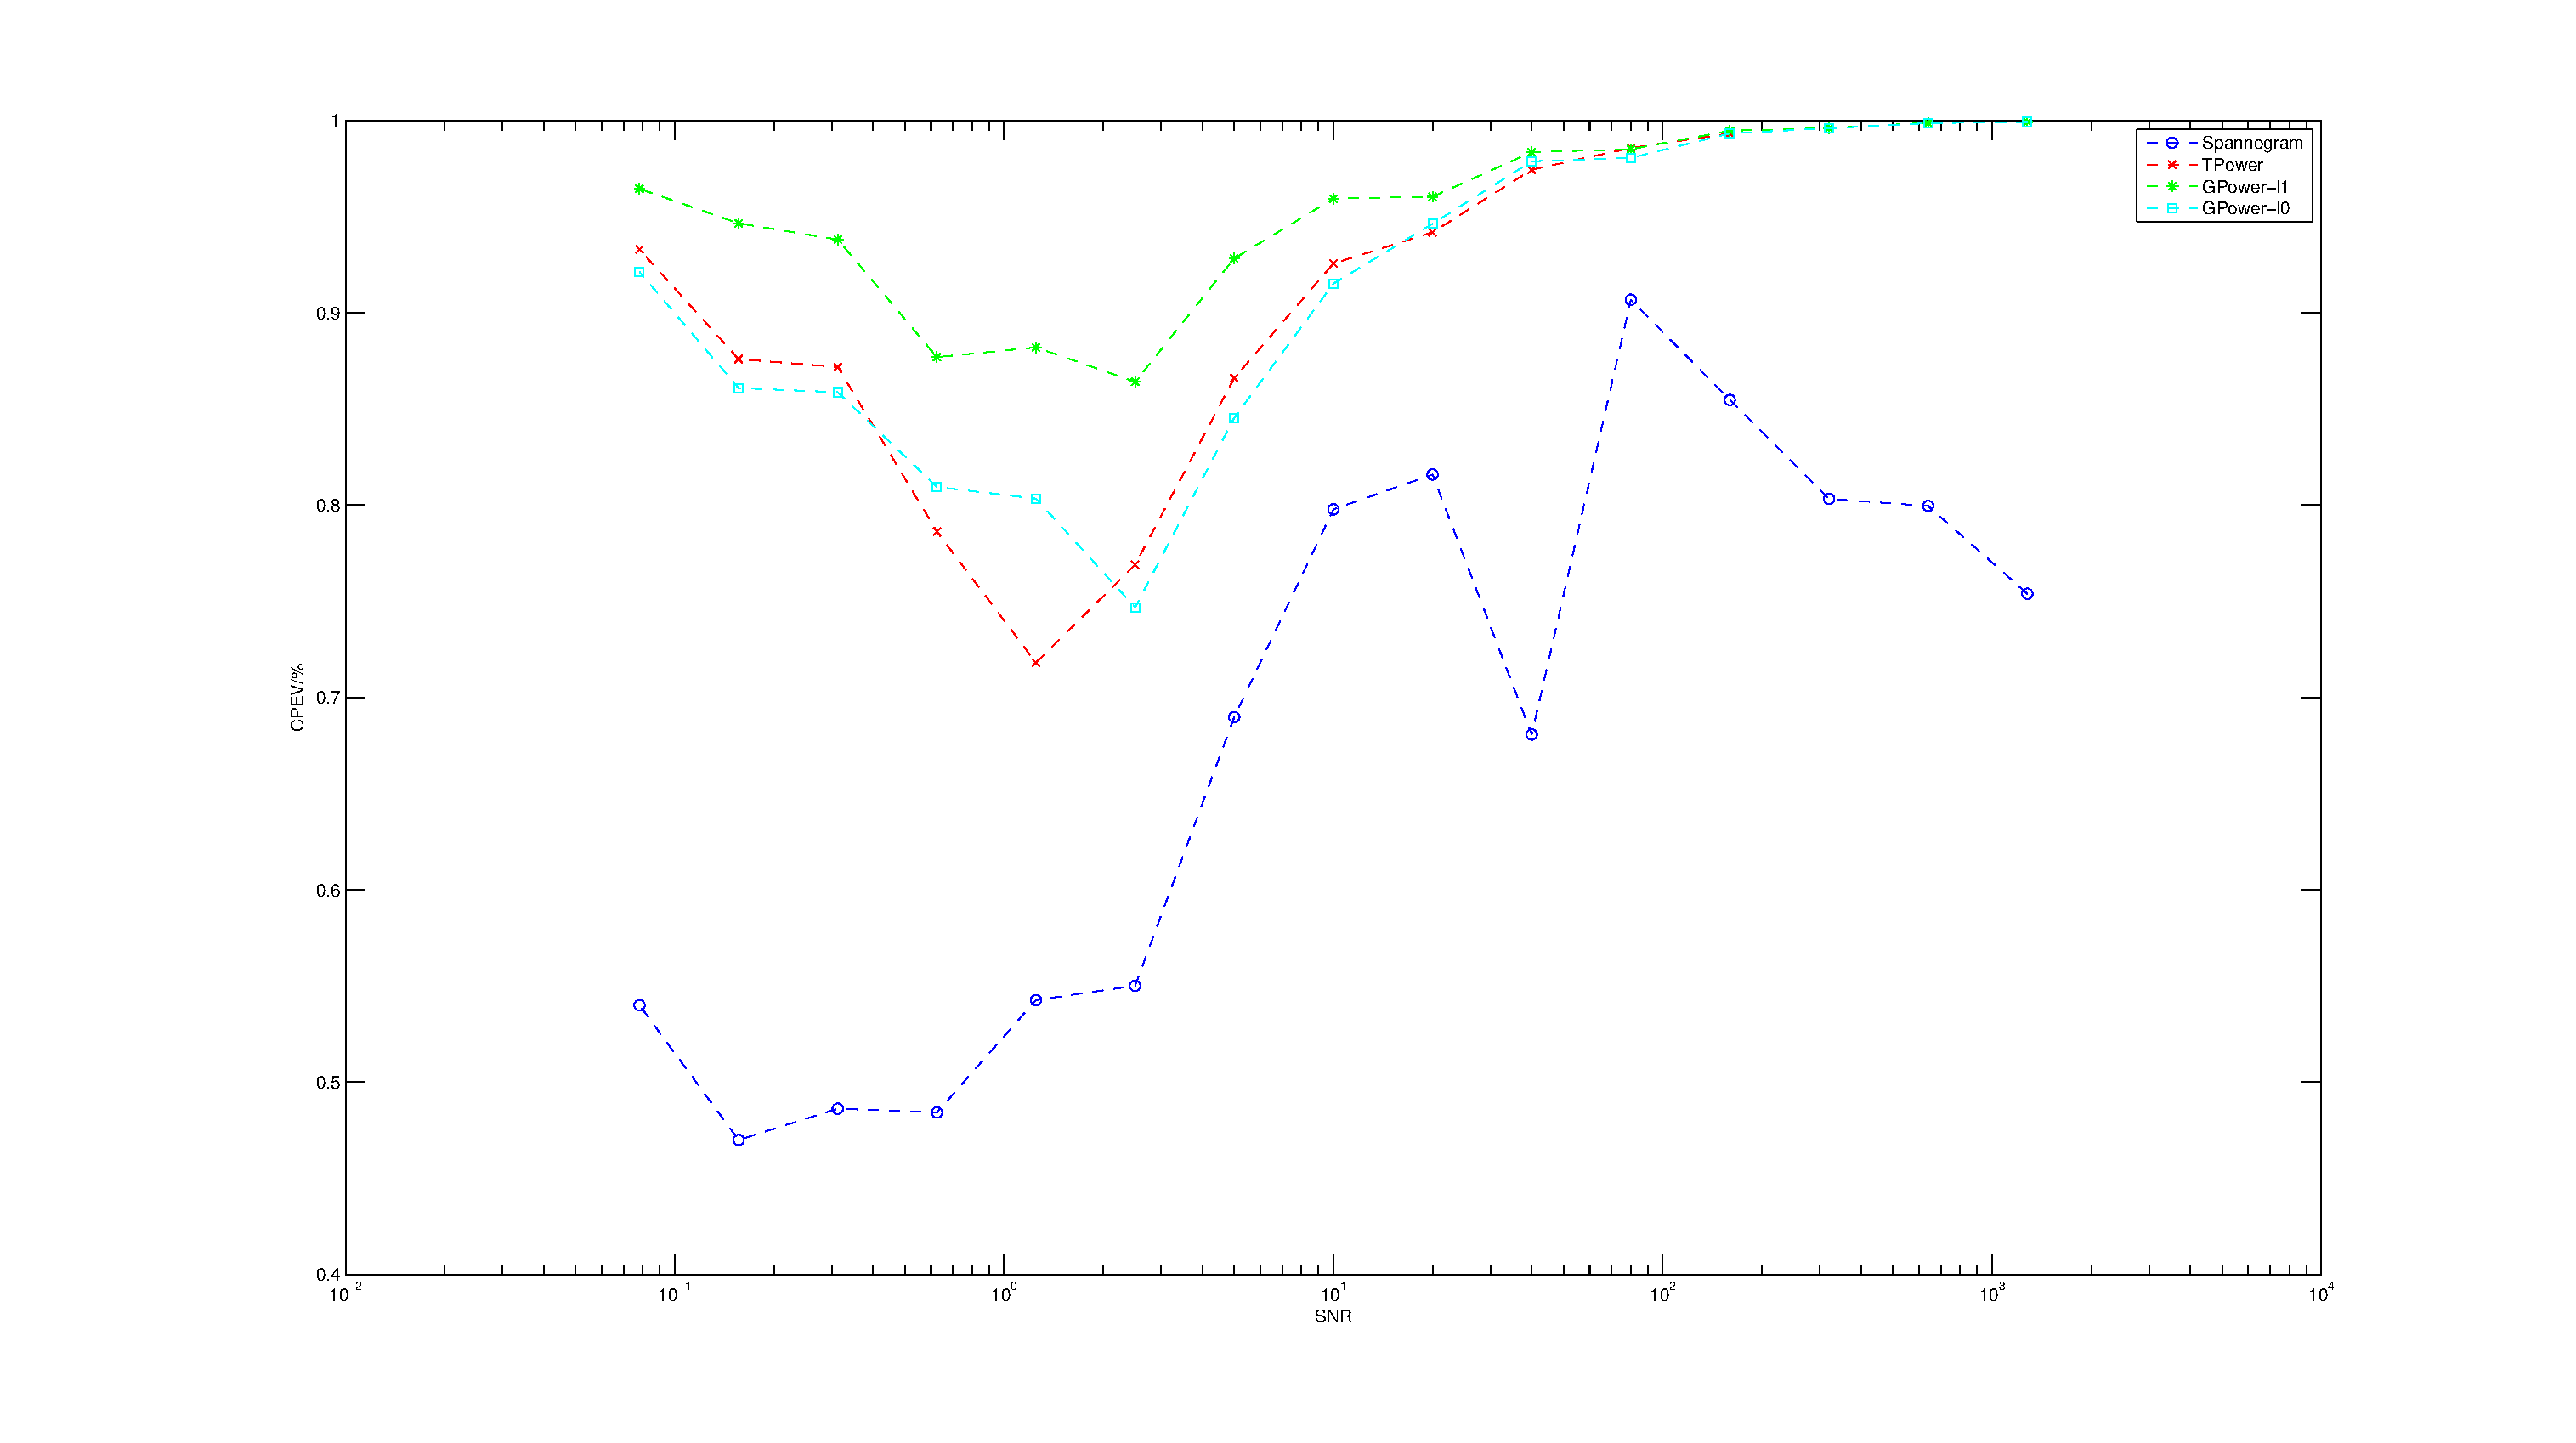
\includegraphics[scale=0.3]{CPEV_10.eps}
\caption{How the different algorithms perform as the SNR varies for fixed sparsity with $m = 10$.}
\label{cpev_10}
\end{figure}

\textbf{***Explain Results***}

It can be seen here that the TPower and GPower algorithms seems to always outperform the Spannogram PCA algorithm considered in \cite{dimakis}, and by a very significant amount for both cases. As is evident in Table \ref{performance_5000}, the TPower algorithm maintains over $80$\% of the variance whereas the Spannogram PCA algorithm captures $12$\% less. This is further shown in Table \ref{performance_10}, where the number of data points is even lower and again there is a gap of roughly $10$\% between the two, TPower being best. Added to this, the average computation time for the Spannogram PCA algorithm is more than $5000$ times slower than that of the TPower method. It should be noted that both algorithms used the deflation method described in \cite{Mackey_deflationmethods} to ensure that, upon calculation of each principal component the covariance matrix can be projected onto a subspace which is not influenced by it.

These results highlight the fact that more work must be done evaluating some of the other algorithms that exist, such as those in \cite{shen}, \cite{zou}, \cite{daspremont} and \cite{asteris} throughout the remaining part of this project.


\subsubsection{Testing with Binary Data Matrix $\smat$}
\begin{comment}
 results can be found in testing_sparse_PCA_binary_matrix_different_levels_sparsity_results.mat
\end{comment}
Though the Spannogram algorithm seems to perform the worst in the scenario above, where the covariance matrix has actual sparse eigenvectors, in \cite{dimakis} the authors do not use it on this type of matrix, and for the specific example that is being considered in this paper initially (Twitter data), the data matrix, $\smat$, is a binary matrix, each entry taking only the values in the set $\{ 0, 1\}$. Furthermore, the matrix $\covmat$ is not equal to a conventional covariance matrix (refer to section \ref{covmat}). This test revolves around trying to emulate this scenario. 

The data matrix, $\smat$, is created by adding a one to each entry independent of any other entry with some probability $p_\text{1}$, which is chosen to be $0.05$, which is quite artificial since it very likely that many features will come in packages, since this is essentially what is being searched for. Nevertheless, this is done and then the covariance matrix, $\covmat$, is created as in section \ref{covmat}. The algorithms are then used on this to find the sparse principal components and the performance score is calculated, as previously. The results can be seen in Figure \ref{perf_score_binary_matrix} and Table \ref{performance_bin_data_5000}. In this case, though all algorithms have quite a low performance, the Spannogram algorithm actually performs the best. 


\begin{table}[H]
\center
\begin{tabular}{|l|r|}
\hline
Algorithm &  Average Computation Time/s\\
\hline
Spannogram-R3 &10.6410\\
TPower &   0.0068\\
GPower-$l_1$  &    0.0151\\
GPower-$l_0$  &   0.0055\\
\hline

\end{tabular}
\caption{Table showing the average computation time of different algorithms for computing sparse principal components of the matrix $\mathbf{A}$ with $m=5000$ for a binary data matrix $\smat$.}
\label{performance_bin_data_5000}
\end{table}

As a further test, the data matrix is created slightly differently. Instead of having all feature's probabilities independent of one another, this time some features are given as correlated. If one of the features in the correlated set is one, then the probability, $p_\text{corr}$, of the rest being one increases drastically, in this case this probability is set to $0.85$. This should give results slightly more relevant to the the scenario of interest since words which are related in some way should appear more frequently together than words that aren't. 

Then different sparsity levels are created by increasing the value of the  $p_\text{1}$, whilst keeping $p_\text{corr}$ constant. The sparsity levels (given as a percentage of how many non-zero elements $\smat$ has) are expected to be slightly higher than $p_\text{1}$ due to the fact that $p_\text{corr}$ will be used occasionally also. 

The features to be correlated are arbitrarily chosen to be feature numbers $1, 2, 31, 39, 40$. 5 have been chosen and the algorithms should all aim to return 5-sparse vectors (for the GPower algorithm this is heuristically set by $\rho$, see \cite{GPower}, and a setting of between 0.3 and 0.5 is used here) corresponding to these. The algorithm is run with $m = 5000$ data points and the $m = 10$ data points is neglected as the relative performance does not seem to change. What can be seen from these results is that both the Spannogram and the TPower algorithm have identical results under these circumstances. As the sparsity ranges from roughly $0.05\%$ to $75\%$ both get the exact same score and identical sparse PCs. On the contrary, both GPower algorithms do significantly worse, and this is largely due to the fact that the tuning parameter $\rho$ must be chosen very carefully for a desired sparsity and this makes it very sensitive to changes in the sparsity of $\smat$. When GPower$_{l1}$ does match the other two, however, it has almost the exact same PCs also, with the same sparsity level. The setting that is being considered in this report is with $\smat$ of $1.5\%$ sparsity or less, as detailed in section \ref{sparsity_matrix}. Due to the fact that the Spannogram Algorithm and the TPower algorithm perform best in this range, according to these results, and the fact that a binary matrix is what is actually considered, as is the case in this section, the GPower algorithms will no longer be used and instead the Spannogram and TPower algorithm will be evaluated against one another. 

\begin{figure}[H]
\centering
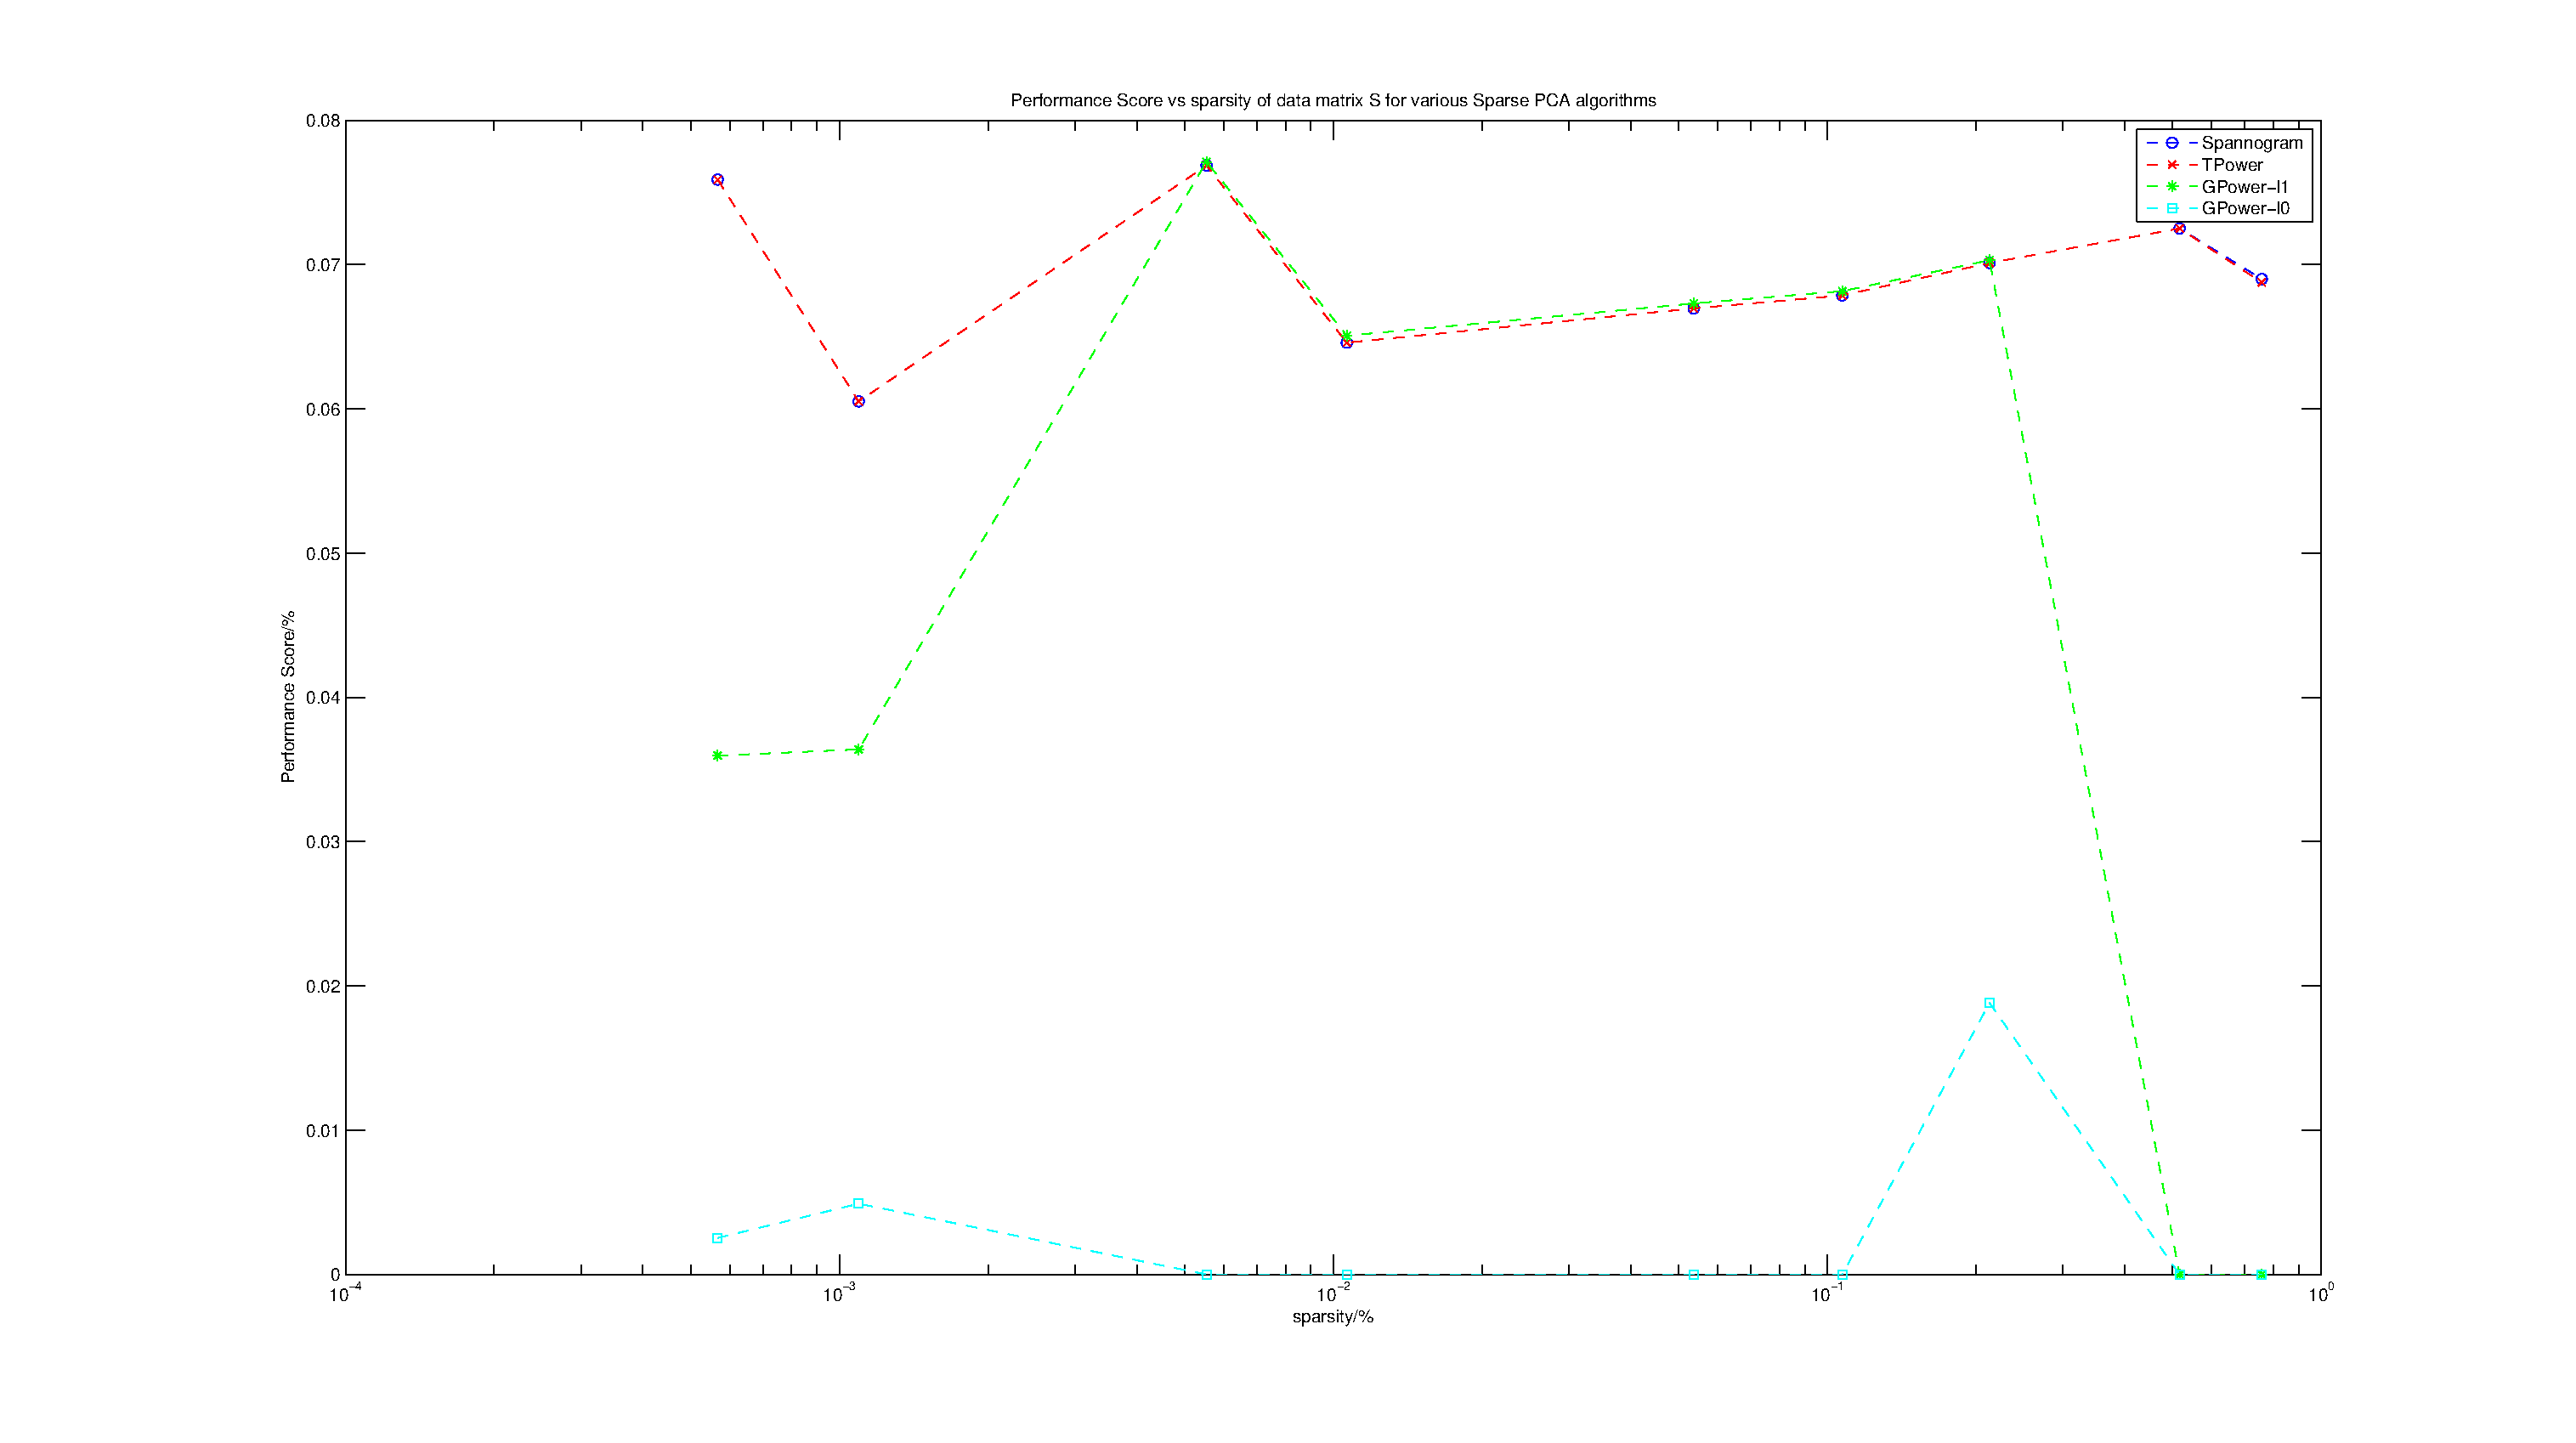
\includegraphics[scale=0.3]{perf_score_binary_matrix.eps}
\caption{How the different algorithms perform as the average sparsity varies with $m = 5000$.}
\label{perf_score_binary_matrix}
\end{figure}

\textbf{TODO}
\begin{itemize}
\item Explain that TPower and Spannogram seem to be the same in performance.
\item Explain that it is difficult to tune GPower with the right value for the $\rho$ parameter so will be discontinued as it keeps giving non-sparse vectors.
\item Explain how the actual eigenvector differs from the sparse eigenvector. 
\end{itemize}

\begin{equation*}
\mathbf{\mathbf{v}_1}=
\begin{pmatrix}
0.1564\\
0.1718\\
0.1567\\
0.1545\\
0.1554\\
0.1577\\
0.1556\\
0.1576\\
0.1557\\
0.1571\\
0.1559\\
0.1585\\
0.1563\\
0.1566\\
0.1569\\
0.1561\\
0.1565\\
0.1563\\
0.1552\\
0.1562\\
0.1566\\
0.1570\\
0.1552\\
0.1568\\
0.1565\\
0.1586\\
0.1554\\
0.1563\\
0.1583\\
0.1568\\
0.1716\\
0.1586\\
0.1579\\
0.1576\\
0.1572\\
0.1559\\
0.1568\\
0.1568\\
0.1695\\
0.1698\\
\end{pmatrix}
\end{equation*}

\subsubsection{Complexities of the Different Algorithms}

\subsection{Testing the Sparse PCA Algorithms on Twitter Data}
\label{testing_twitter}
The file used to test the Spannogram PCA algorithm contains all the Tweets in the London area from 23rd September 2012 to the 2nd October 2012. It has been partitioned into 10 files, each containing roughly 40k Tweets, which corresponds to about a day of Tweets for each file.

\begin{table}[H]
\center
\begin{tabular}{| c l |}
\hline
Index & Word \\
\hline
134 & terry\\
133 & john\\
79 & football\\
334 & international\\
157 & england\\
921 & retires\\
\hline
\end{tabular}
\caption{The dominant principal component for 23/09/2012 - 24/09/2012.}
\label{john_terry}
\end{table}

\begin{table}[H]
\center
\begin{tabular}{| c l |}
\hline
Index & Word \\
\hline
24 & please\\
258 & following\\
842 & officers\\
904 & murders\\
798 & fallen\\
204 & police\\
\hline
\end{tabular}
\caption{The dominant principal component for 25/09/2012 - 26/09/2012.}
\label{murder}
\end{table}

\begin{table}[H]
\center
\begin{tabular}{| c l |}
\hline
Index & Word \\
\hline
41 & europe\\
17 & rydercup\\
6 & come\\
2 & well\\
95 & rydercup2012\\
26 & done\\
\hline
\end{tabular}
\caption{The dominant principal component for 30/09/2012 - 01/09/2012.}
\label{ryder_cup}
\end{table}

Clearly, Table \ref{john_terry} refers to the retirement of England's former captain, John Terry, from international football, which can be confirmed by the Daily Mail on the 23rd September 2012 and The Guardian on the 24th September 2012. Table \ref{murder}, on the other hand, is a result of a trending Tweet regarding a murder that took place on the 19th September 2012, where 2 police officers were killed. The final principal component, visible in Table \ref{ryder_cup}, emerges as a result of Europe's victory over the US in the Ryder Cup golf competition in 2012. 

These are the most interesting principal components that appear from running the algorithm on the data, however some others also come up, which are associated with advertisements. Some batches, contrariwise, did not have any relevant principal components, which is a result of there not being any significant event that took place during the associated time periods.

\subsection{Illustration using TPower and Spannogram PCA}
To test the performance of the TPower algorithm and the Spannogram algorithm for the Twitter data gathered for the period 25/09/2012 - 26/09/2012 different sparseness is considered for the principal components and the first two principal components are evaluated by the algorithms. 

The set of words that is desired can be seen in Table \ref{murder_8} as these are the words that represent the most significant event that happened in the period of time considered. Let this set be referred to as $S$. Other sparse principal components do emerge, however, they mostly arise as words that may occur quite frequently together but do not actually represent a specific event, for instance ``happy'' and ``birthday'' appear quite  a lot, but do not actually represent a single event. 

\begin{table}[H]
\center
\begin{tabular}{| c l |}
\hline
Index & Word \\
\hline
12 & please\\
756 & recent\\
787 & colleagues\\
240 & following\\
827 & officers\\
889 & murders\\
783 & fallen\\
190 & police\\
\hline
\end{tabular}
\caption{The dominant 8-sparse principal component for 25/09/2012 - 26/09/2012 calculated using the Spannogram PCA algorithm.}
\label{murder_8}
\end{table}


\begin{table}[H]
\center
\begin{tabular}{|c|r|r|r|r|}
\hline
 & \multicolumn{2}{ |c|}{TPower } & \multicolumn{2}{ |c|}{Spannogram }\\
\hline
Sparsity& PC1 & PC2 & PC1 & PC2\\
\hline
4& 77.51 & 155.56 & 104.5 & 158.14\\
5& 87.00 & 83.84 & 138.00 & 162.15\\
6& 95.14 & 97.44 & 171.67 & 162.64\\
7& 107.53 & 103.07 & 205.44 & 165.98\\
8& 117.11 & 239.25 & 239.26 & 165.91\\
\hline
\end{tabular}
\caption{Explained variance captured by first two principal components calculated by the TPower algorithm and the Spannogram algorithm.}
\label{explained_var_table}
\end{table}

\begin{figure}[H]
\centering
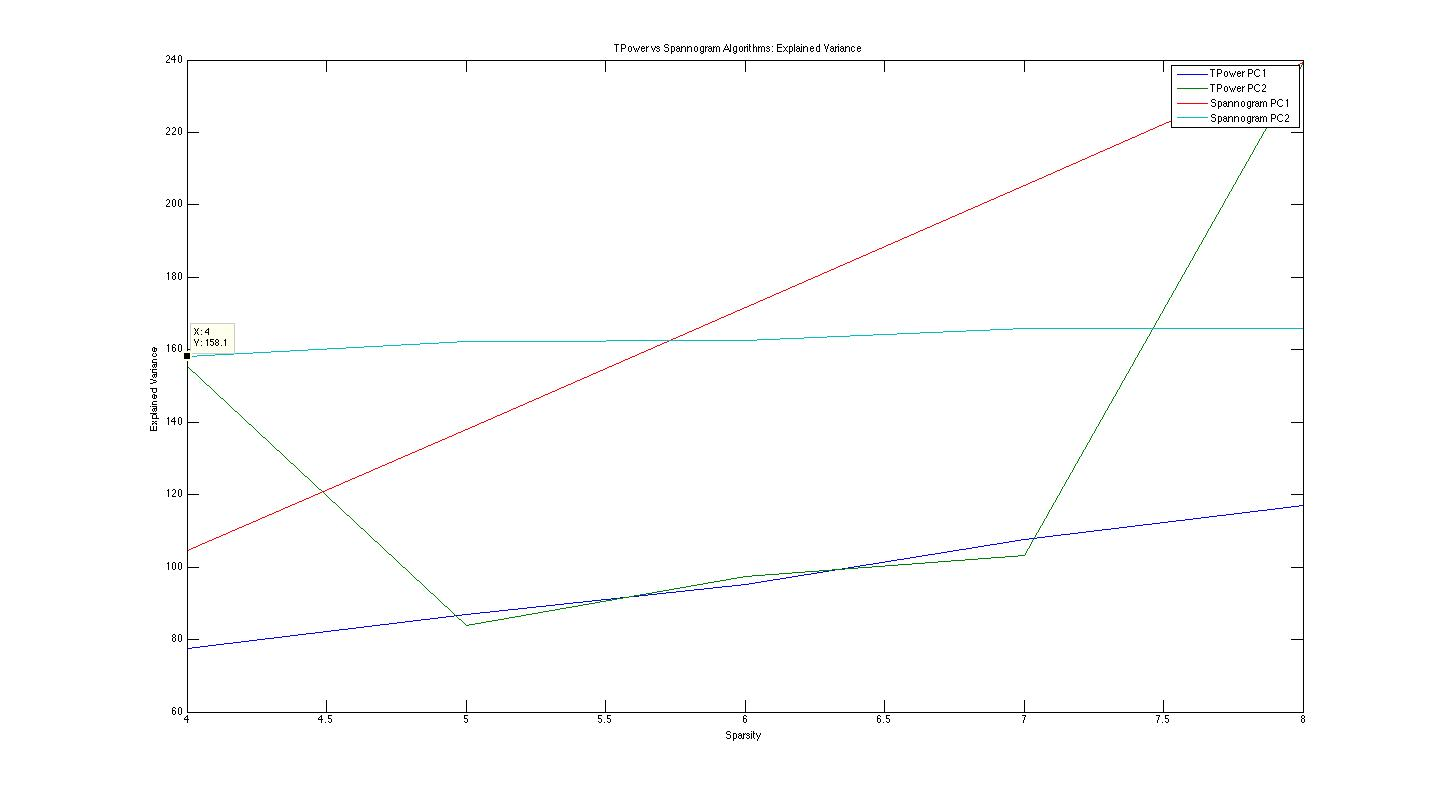
\includegraphics[scale=0.3]{TPower_VS_Spannogram.jpg}
\caption{How the explained variance of the principal components varies with the sparsity.}
\label{explained_var_graph}
\end{figure}



As shown in Table \ref{explained_var_table} and Figure \ref{explained_var_graph} the Spannogram PCA algorithm always outperforms the TPower algorithm for both principal components (PC). The interesting thing to note from these is that (a) the TPower algorithm is not consistent in its findings, as can be seen by its second PC, which initially has quite a high value and one of the words from $S$, but after increasing the value of k, fails to have any of the words in $S$ until k becomes 8, at which point it contains all the words in $S$. The Spannogram algorithm on the other hand consistently keeps its previously calculated words and, upon each increase in sparsity, it just adds an extra word. Furthermore, for the Spannogram algorithm, the explained variance associated with both PCs monotonically increase with respect to the sparsity, which is not the case for the TPower algorithm, the red line in the figure increasing the most since it is associated with the words in Table \ref{murder_8}.

These results are completely contrary to the results found in section \ref{testing}. This is largely believed to be accounted for by the structure of the $\mathbf{S}$ matrix in each case. In \cite{truncpower}, it is suggested that if the matrix $\mathbf{A}$ has sparse or approximately sparse eigenvectors then the TPower algorithm can approximate these, which has as its underlying assumption that the true eigenvectors are themselves almost sparse. The Spannogram algorithm does not make this assumption at all. Instead it finds PCs which may not represent the true PCs in any way whatsoever. For instance, getting the true leading eigenvector of $\mathbf{A}$, it turns out to be that 44 of the 3000 words are at least $50\%$ the magnitude of the highest magnitude element in the leading eigenvector. Which may be approximately sparse considering that this is a small fraction of 3000 but it is still much larger than just 4 to 8 words. In this context, the vector is not sparse at all. This is a crude measurement for ``approximately'' sparse but it is merely for illustration purposes. 

It can be concluded that the Spannogram PCA algorithm performs best when the matrix $\mathbf{A}$ does not actually have sparse PCs in the conventional sense but still has sparse components that can model the variance in the data fairly well. 

\subsection{Conclusion}

\clearpage



\section{Further Implementation and Evaluation}
\begin{comment}
From the results found so far, it can be seen that different algorithms may prove to be more effective than the Spannogram PCA algorithm. This means that further work has to be done evaluating other algorithms, as those found in \cite{shen}, \cite{zou}, \cite{daspremont}, \cite{asteris} 
and any others, and finding which ones would be best to use for the specific scenario. It may be the case that the Spannogram PCA algorithm performs worse with a conventional covariance matrix, but performs much better on the matrix $\mathbf{S}^T\mathbf{S}$ which is used on the Twitter data, so this also must be researched further. 

The algorithms will be evaluated, as done in section \ref{testing}, and a performance score will be given to them. Then the same algorithms will be evaluated on the Twitter data, as in section \ref{testing_twitter} and the results will be compared to see whether algorithm performances depend on the data structure. The results of this research will lead to an algorithm being chosen and this algorithm will be examined further so as to find any improvements that could be made to it, or a couple of algorithms could be merged to keep the benefits of both. Consideration will also be given to the data at hand to see if the structure could be exploited further, as the authors of \cite{dimakis} attempt to do. Upon completion of this, the new algorithm will also be evaluated similarly to before, to determine whether the alterations have had a positive effect.

If along the way any other difficulties arise, due to scalability issues or the data structure, these will first be tackled and the changes will also be evaluated. 

\end{comment}

\subsection{Big Data Streaming Applications}
In this section, methods to ensure computational feasibility are considered, and an algorithm is created to make this possible under high volume data applications in which the rate of data is very large while the number of variables considered is comparatively low i.e. $m >> n$. As already mentioned previously, there are roughly 40k Tweets on average per day in London, which corresponds to quite a small volume which can be processed all in one go, but suppose that the world were to instead be considered, which would give a rate of about 58 million Tweets per day, then clearly a method would need to be considered to be able to process all that data in a streaming fashion. 

Needless to say, this would only work if there were an actual trending topic in the whole of the population. 

The algorithm can be described as follows.

\RestyleAlgo{boxruled}
\LinesNumbered
\begin{algorithm}[H]
\KwData{The Stream of Tweets}
\KwResult{The Sparse Principal Components for each batch of Tweets}
\While{Streaming} {
// Calculate the new covariance matrix $\covmat = \smat\tp \smat$\\
$\smat_\text{new} \leftarrow $ New Batch of $K$ Tweets;\\
// Pop the old data off the queue, $\mathbf{Q}$\\
$\smat_\text{old} \leftarrow \mathbf{Q}(1:K)$;\\
// Shift the queue of data. W is the sliding window size.\\
$ \mathbf{Q}(1:W-K) \leftarrow \mathbf{Q}(K+1:W) $\\
// Put the new data at the end of the queue\\
$ \mathbf{Q}(W-K+1:W) \leftarrow \smat_\text{new}$\\
// Calculate the new covariance matrix using the old covariance matrix,\\
// the old data and the new data\\
$\covmat_\text{new} \leftarrow \covmat_\text{old} - \sum_{j = 1}^K \left[\smat_\text{old}\right]_{i,:}\tp\left[\smat_\text{old}\right]_{i,:} + \sum_{j = 1}^K \left[\smat_\text{new}\right]_{i,:}\tp\left[\smat_\text{new}\right]_{i,:}$\\ 
// Check whether old PCs are valid or whether new ones must be calculated\\
\If{OldPCsValid($\covmat_\text{new}$, $\mathbf{V}_\text{old}$, $\mathbf{\Lambda}_\text{old}$)} 
{$[\mathbf{V}_\text{new}, \mathbf{\Lambda}_\text{new}] = [\mathbf{V}_\text{old}, \mathbf{\Lambda}_\text{old}]$}
\Else {
	$[\mathbf{V}_\text{new}, \mathbf{\Lambda}_\text{new}]$ = ComputeSparsePCA($\covmat_\text{new}$);
}
ListOfSparsePCs.Append($\mathbf{V}_\text{new}$)\\
ListOfEigenvalues.Append($\mathbf{\Lambda}_\text{new}$)\\
$[\mathbf{V}_\text{old}, \mathbf{\Lambda}_\text{old}] = [\mathbf{V}_\text{new}, \mathbf{\Lambda}_\text{new}]$
}
\end{algorithm}

The OldPCsValid function checks whether the old Sparse Principal Components are still valid by checking what the percentage of variance explained by them is and how this has has changed since the previous iteration, if this has changed significantly from the last batch or it falls beneath a certain (heuristic) threshold, then new Sparse PCs are computed using the algorithm of choice. 

Computation time is saved in two ways. Firstly, the covariance matrix doesn't need to be computed directly every single time. This is significant if the window size, $W$, is much larger than the batch size, $K$, reducing it from $O(Wn^2)$ to $O(Kn^2)$, which is not a major improvement but still makes a difference. The most significant improvement is seen in the validation of the old principal components. This does a quick check to see whether the variance explained by the Sparse PCs still qualifies them to be the dominant components and, if so, the algorithm doesn't actually have to be implemented for that particular iteration, saving computation time. This means that, on average, for a buffered streaming input, the output rate of PCs can increase for much smaller batches. The great thing about this is that smaller batches means better resolution in time and it means that for large volume applications that the algorithm will terminate much faster. 

\subsection{Financial Application: Hedging}

\subsection{Bayesian Networks: Pearl's Algorithm}
\clearpage

\bibliography{bibliography}
\bibliographystyle{plain}
\clearpage

\section*{Appendix}\label{appendixa}

\appendix
\pagenumbering{Roman}

\section*{A. PCA Explained (A variant of \cite{bishop})}

Consider a set of observations $\{\mathbf{x}x_n\}$ for $n = 1, ..., N$ and each $\mathbf{x}_n \in \mathbb{R}^D$, to project the data onto just one dimension whilst keeping the maximum amount of variation possible (and therefore information), we can project the data onto one D-dimensional vector, $\mathbf{u}_1 \in \mathbb{R}^D$. The mean of the projected data is then $\mathbf{u}_1^T \mathbf{\overline{x}}$, where
\begin{equation*}
\mathbf{\overline{x}} = \frac{1}{N} \sum_{n = 1}^N \mathbf{x}_n 
\end{equation*} 
the sample mean of the observed data.

The sample variance of the projected data can then be given by
\begin{equation*}
\frac{1}{N} \sum_{n = 1}^N \{\mathbf{u}_1^T\mathbf{x}_n -  \mathbf{u}_1^T\mathbf{\overline{x}}_n\}^2
\end{equation*} 
\begin{equation*}
\mathbf{u}_1^T \left( \frac{1}{N} \sum_{n = 1}^N \left(\mathbf{x}_n - \mathbf{\overline{x}}_n\right)\left(\mathbf{x}_n - \mathbf{\overline{x}}_n\right)^T \right) \mathbf{u}_1
\end{equation*} 

Taking notice that 
\begin{equation*}
\frac{1}{N} \sum_{n = 1}^N \left(\mathbf{x}_n - \mathbf{\overline{x}}_n\right)\left(\mathbf{x}_n - \mathbf{\overline{x}}_n\right)^T 
\end{equation*} 
is just the covariance matrix of the data, call it $\mathbf{S}$, we can the say that:
\begin{equation}
\mathbf{u}_1^T \mathbf{S} \mathbf{u}_1
\label{uSu}
\end{equation} 

Therefore, if we would like to maximise the variance of the projected data, we need to maximise \eqref{uSu}. This can obviously be maximised by letting $\|\mathbf{u}_1\| \to \infty$, without taking into account the actual direction of $\mathbf{u}_1$, however this is not what is desired. What is actually needed is the direction in which the data varies most and not the actual length of the vector itself. A constraint is therefore imposed such that $\|\mathbf{u}_1\| = 1$ and then a Lagrange multiplier is introduced, $\lambda_1$. The resulting equation is as such:


\begin{equation*}
\mathbf{u}_1^T \mathbf{S} \mathbf{u}_1 - \lambda_1 (1 - \mathbf{u}_1^T \mathbf{u_1})
\label{lagrange_uSu}
\end{equation*} 

Which by setting the derivative with respect to $\mathbf{u}_1$ to zero, the following is attained:


\begin{equation*}
\mathbf{S} \mathbf{u}_1 = \lambda_1  \mathbf{u_1}
\label{eig_uSu}
\end{equation*} 

Which means that $\mathbf{u}_1$ is maximised by finding the eigenvector with the largest eigenvalue $\lambda_1$. Similarly to find the $M$ principal components, the eigenvectors of the covariance matrix with the $M$ highest eigenvalues must be calculated.
\clearpage
\section*{B. Useful Intuition for the Covariance Matrix $\mathbf{A}$}
Consider a matrix, $S\in \mathbb{R}^{m\times n}$, where $m$ is the number of Tweets and $n$ is the number of features that the tweets are evaluated on, in this case the Bag-of-Words. Performing $S^TS = A$ where $A \in \mathbb{R}^{n\times n}$. 

By example, imagine:

\begin{equation}
S = \left( \begin{matrix}
a_{1, 1} & a_{1, 2} & a_{1, 3} \\ 
a_{2, 1} & a_{2, 2} & a_{2, 3} \\
a_{3, 1} & a_{3, 2} & a_{3, 3} \\
a_{4, 1} & a_{4, 2} & a_{4, 3} 
\end{matrix} \right)
\end{equation}

\begin{equation}
A = S^TS =
 \left( \begin{matrix}
a_{1, 1} & a_{2, 1} & a_{3, 1} & a_{4, 1} \\ 
a_{1, 2} & a_{2, 2} & a_{3, 2} & a_{4, 2} \\ 
a_{1, 3} & a_{2, 3} & a_{3, 3} & a_{4, 3} \\ 

\end{matrix} \right)
\cdot \left( \begin{matrix}
a_{1, 1} & a_{1, 2} & a_{1, 3} \\ 
a_{2, 1} & a_{2, 2} & a_{2, 3} \\
a_{3, 1} & a_{3, 2} & a_{3, 3} \\
a_{4, 1} & a_{4, 2} & a_{4, 3} 
\end{matrix} \right)
\end{equation}


\begin{equation}
A =
\left( \begin{matrix}
\sum_{i=1}^4 a_{i,1}^2& \sum_{i=1}^4 a_{i,1} a_{i,2} &  \sum_{i=1}^4 a_{i,1} a_{i,3} \\ 
\sum_{i=1}^4 a_{i,2}a_{i, 1} & \sum_{i=1}^4 a_{i,2}^2 &  \sum_{i=1}^4 a_{i,2} a_{i,3} \\ 
\sum_{i=1}^4 a_{i,3}^2& \sum_{i=1}^4 a_{i,3} a_{i,2} &  \sum_{i=1}^4  a_{i,3}^2 \\ 
\end{matrix} \right)
\end{equation}

Since $a_{i, j} = 1$ when the word $j$ appears in Tweet $i$ and otherwise 0, the resulting matrix is basically a symmetric matrix with entry $(i, j)$ being composed of the number of times word $j$ occurs with word $i$ in the same Tweet over all the Tweets. The diagonal is  therefore the number of times the word $j$ appears over all the Tweets.

This is basically a form of clustering i.e. words that occur frequently together will have high corresponding values in the matrix $A$.  


\end{document}
